\title{Tecnologie Web}
\maketitle

\chapter{HTTP}
\section{Protocolli di rete}
Un protocollo è una definizione formale di un comportamento esterno per una entità comunicante. Definisce formato, ordine dei messaggi ricevuti e inviati e le azioni prese alla ricezione e trasmissione di un messaggio. \\

Un protocollo è \textbf{orientato alla connessione, connection oriented} se le entità peer devono essere sincronizzate prima di scambiarsi dati utili (connessione impostata); altrimenti è \textbf{non orientato alla connessione, cioè connectionless}.

\subsection{Strati dei protocolli}
Le funzioni di rete sono strutturate come un modello a strati:
\begin{itemize}
    \item lo strato \emph{n} comunica con l'altro strato \emph{n}; i dati scambiati sono chiamati \textbf{Protocol Data Unit (PDU)}
    \item lo strato \emph{n} usa il \textbf{servizio} dello strato $n - 1$ e offre un servizio allo strato $n + 1$; i dati di interfaccia sono chiamati \textbf{Service Data Unit (SDU)}
    \item entità allo stesso livello sono denotate come \textbf{peer entities}
    \item le regole di funzionamento tra peer entities sono chiamate \textbf{procedures}
\end{itemize}

\begin{center}
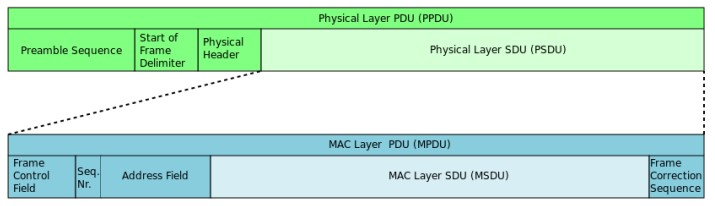
\includegraphics[scale=0.4]{Images/TecnologieWeb/1/4.jpg}    
\end{center}

\subsubsection{Perchè usare la stratificazione?}
La struttura esplicita permette la identificazione e le relazioni tra parti di sistemi complessi. La modularità facilità il mantenimento e l'aggiornamento di un sistema: un cambiamento nella implementazione di un servizio di uno strato è trasparente rispetto al resto del sistema.

\subsection{Stack dei protocolli internet}
\begin{itemize}
    \item Applicazione: supporta le applicazioni di rete $\rightarrow$ FTP, SMTP, HTTP
    \item Trasporto: trasferimento dati tra processi $\rightarrow$ TCP, UDP
    \item Rete: instradamento dei datagrammi dalla sorgente alla destinazione $\rightarrow$ IP, protocolli di routing
    \item Link: trasferimento dati tra elementi di reti adiacenti $\rightarrow$ Ethernet, 802.11 (WiFi), PPP
    \item Fisico: bits "on the wire"
\end{itemize}

\section{Incapsulamento}
\begin{center}
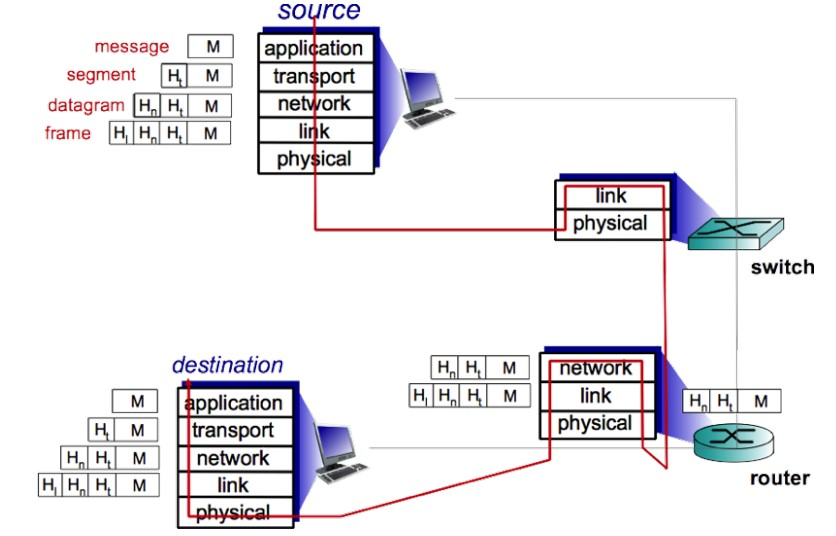
\includegraphics[scale=0.4]{Images/TecnologieWeb/1/encapsulation.jpg}
\end{center}


\section{Servizi di rete (Network services)}
Un servizio di rete è una applicazione basata su protocolli di rete a livello applicazione. Esempi sono: name service (DNS), mail (SMTP), web (HTTP), ecc... \\

Esempio con due network services: name e web
\begin{center}
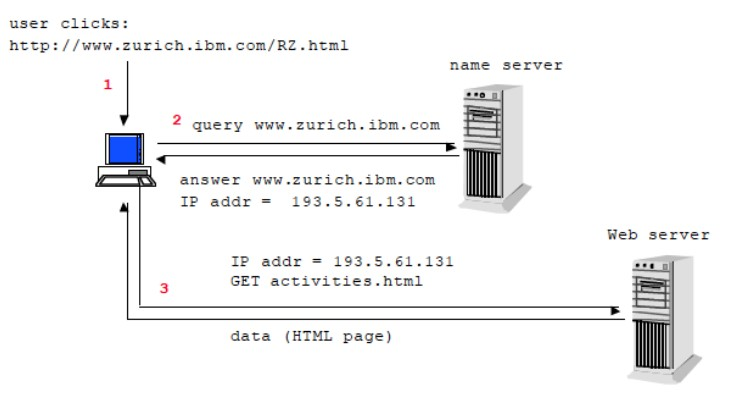
\includegraphics[scale=0.4]{Images/TecnologieWeb/1/networkservices.jpg}    
\end{center}

\section{Creazione di un servizio di rete}
Scrivere un programma che:
\begin{itemize}
    \item viene eseguito su diversi \textbf{end systems}
    \item comunica sulla rete
\end{itemize}

End$-$to$-$end principle: i dispositivi centrali della rete non eseguono/forniscono servizi di rete.

\section{Processi comunicanti}
\textbf{Processo}: programma eseguito in un host
\begin{itemize}
    \item nello stesso host, due processi comunicano usando \textbf{inter-process communication} definita dal sistema operativo
    \item processi in host diversi comunicano scambiando \textbf{messaggi}
\end{itemize}

\textbf{Client process}: processo che inizia la comunicazione
\textbf{Server process}: processo che aspetta di essere contattato 

\section{Sockets}
Una socket è un endpoint in un collegamento di comunicazione bidirezionale tra due programmi in esecuzione su una rete. Una socket è legata a un numero di porta tale per cui il livello di trasporto può identificare la applicazione per cui certi dati sono destinati.

\begin{center}
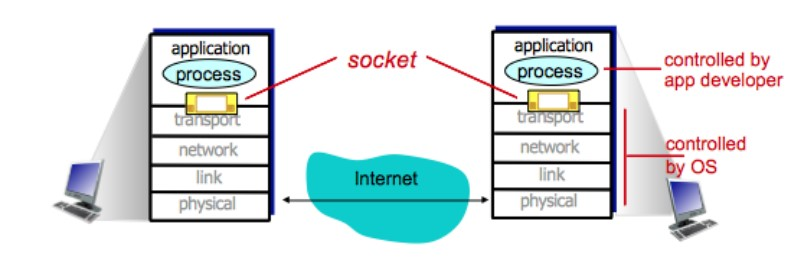
\includegraphics[scale=0.4]{Images/TecnologieWeb/1/Sockets.jpg}    
\end{center}

\section{Indirizzamento (Addressing)}
Per ricevere messaggi, un processo deve avere un \textbf{identificativo}. Quest'ultimo include sia l'\textbf{indirizzo IP} che il \textbf{numero di porta} associato a un determinato processo. 

\section{Architettura client-server}
Server:
\begin{itemize}
    \item host sempre acceso
    \item indirizzo IP permanente
    \item centri dati per ridimensionamento
\end{itemize}

Client:
\begin{itemize}
    \item comunica col server
    \item potrebbe essere collegato a intermittenza
    \item potrebbe avere indirizzi IP dinamici
    \item non comunicano direttamente tra di loro
\end{itemize}


\section{Peer-to-peer (P2P) architecture}
Non ci sono host sempre accesi (always$-$on), ci sono i peer che rappresentano sia i client che i server in quanto richiedono e forniscono servizi da/a altri peer. La \textbf{autoscalabilità (self scalability)} significa che nuovi peer portano sia nuove capacità di servizi sia nuove richieste di servizi già presenti.
I peer sono connessi a intermittenza e variano gli indirizzi IP per cui la gestione è complessa. 


\section{Trasmission Control Protocol (TCP)}
Inventato da Kahn e Cerf nel 1973. Fornisce:
\begin{itemize}
    \item \textbf{Trasporto affidabile} tra il processo mittente e quello ricevente
    \item \textbf{Controllo di flusso}: il mittente non potrà sovraccaricare il ricevitore
    \item \textbf{Controllo di congestione}: regolare il mittente quando la rete è satura
\end{itemize}
Non fornisce il timing, un throughput minimo garantito, sicurezza. 
\'E un protocollo \textbf{orientato alla connessione} per cui è necessario stabilire un accordo tra le parti.

\section{User Datagram Protocol (UDP)}
Trasferimento dati non affidabile tra i processi comunicanti. Non fornisce: affidabilità, controllo di flusso, controllo di congestione, timing, throughput garantito, sicurezza, impostazione di connessione. 

\begin{center}
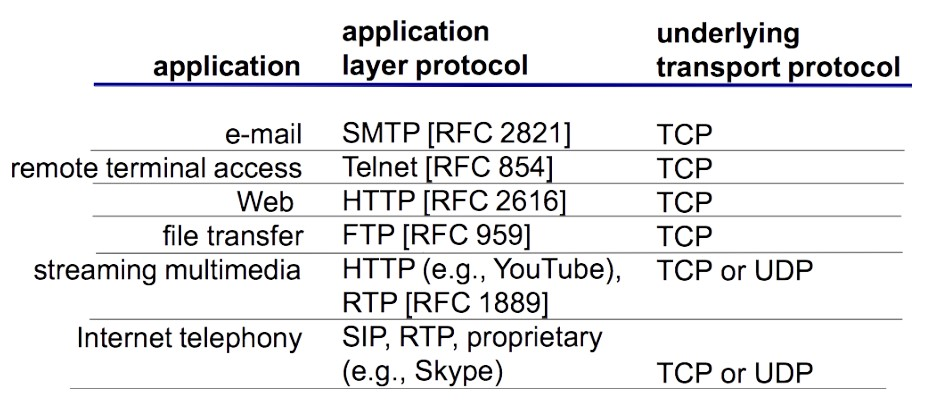
\includegraphics[scale=0.4]{Images/TecnologieWeb/1/NetworkServicesAndTransportProtocols.jpg}    
\end{center}

\section{World Wide Web}
\'E uno spazio di informazioni basato su internet dove i documenti e altre risorse sono identificate da indirizzi. Una pagina web è un documento HTML che è collegato a un'altra pagina web o a risorse.

\section{Uniform Resource Identifiers (URIs)}
La forma del Generic Uniform Resource Identifier (URI) è la seguente:
\begin{center}
    scheme:[//[user:password@]host[:port]][/]path[?query][\#fragment]
\end{center}
Gli URI sono usati da HTTP per identificare le risorse. Nel contesto del WWW, sono informalmente denotati come Uniform Resource Locators (URLs).
\begin{center}
    http://www.example.com/hello.txt
\end{center}
Dove:
\begin{itemize}
    \item http $\rightarrow$ protocollo
    \item www.example.com $\rightarrow$ host name
    \item /hello.txt $\rightarrow$ risorsa
\end{itemize}

\section{Panoramica di HTTP}
\'E un protocollo a livello applicativo e adotta un modello client/server:
\begin{itemize}
    \item \textbf{user agent}: il client che inizia la connessione HTTP e manda la richiesta (HTTP) ad esempio un browser
    \item \textbf{origin server}: programma che accetta (o rifiuta) le connessioni HTTP e possiede le risorse richieste
\end{itemize}
Si hanno poi altre componenti con diversi nomi:
\begin{itemize}
    \item \textbf{local cache}: memoria locale (sia il client che il server potrebbero averla)
    \item \textbf{proxy}: applicazione intermediaria avente sia le funzionalità del client che del server
    \item \textbf{gateway}: applicazione intermediaria che agisce per conto del server (per non avere a che fare direttamente con lui)
\end{itemize}
\hfill \break
\textbf{HTTP usa TCP} quindi:
\begin{enumerate}
    \item il client inizializzza la connessione TCP (crea la socket) col server, porta 80
    \item il server accetta la connessione TCP dal client
    \item i messaggi HTTP sono cambiati tra il browser (HTTP client) e il web server (HTTP server)
    \item la connessione TCP viene chiusa
\end{enumerate}
Inoltre, HTTP è \textbf{stateless} ovvero il server non mantiene alcuna informazione riguardo le vecchie richieste del client. I protocolli che mantengono lo stato sono molto più complessi poichè, ad esempio, nel caso di crash del server, lo stato della connessione potrebbe essere inconsistente.

\section{HTTP non persistente}
Supponiamo che l'utente inserisca il seguente URI:
\begin{center}
    www.someSchool.edu/someDepartment/home.index
\end{center}
\begin{center}
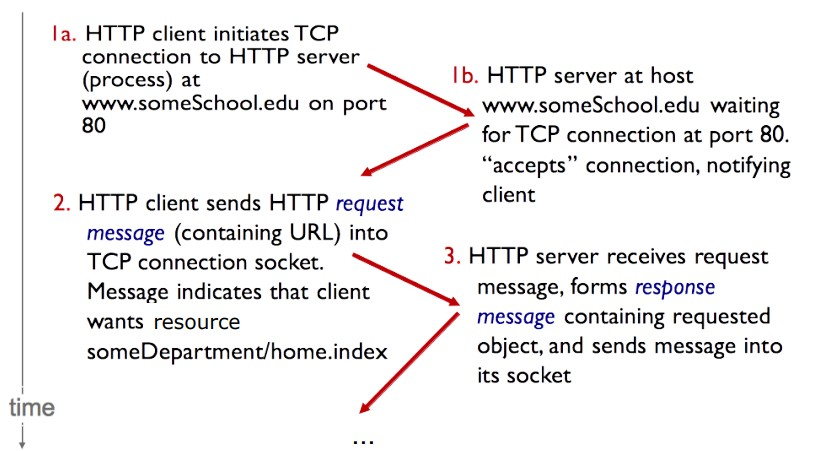
\includegraphics[scale=0.4]{Images/TecnologieWeb/1/NonPersistentHTTP1.jpg}    
\end{center}
\begin{center}
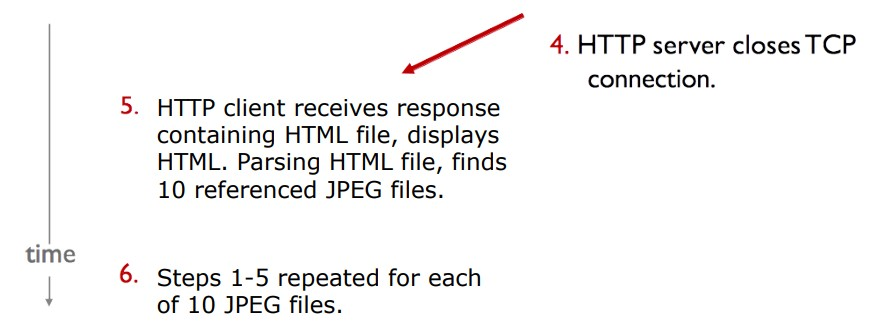
\includegraphics[scale=0.39]{Images/TecnologieWeb/1/NonPersistentHTTP2.jpg}    
\end{center}
In generale, i tempi della connessione sono i seguenti:
\begin{center}
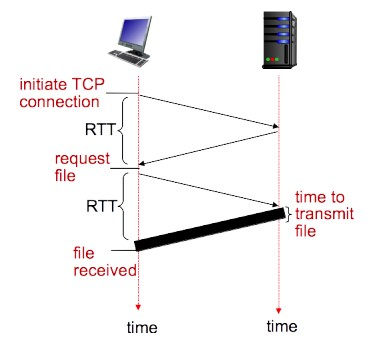
\includegraphics[scale=0.4]{Images/TecnologieWeb/1/RTT.jpg}    
\end{center}
Dove:
\begin{itemize}
    \item Il \textbf{Round Trip Time (RTT)}: tempo necessario a un piccolo pacchetto per viaggiare dal client al server e tornare indietro
    \item Il \textbf{Response time}: un RTT per iniziare la connessione TCP, un altro RTT per la richiesta HTTP e i primi byte di risposta HTTP e il tempo di trasmissione del file
    \item \textbf{Problemi di HTTP non persistente}: \textbf{richiede 2 RTT per ogni risorsa}, c'è un overhead del SO per ogni connessione TCP, il browser spesso apre più connessioni TCP in parallelo  
\end{itemize}


\section{HTTP persistente}
Il server lascia la connessione aperta dopo aver mandato la risposta per cui i messaggi HTTP successivi riutilizzano quella connessione, risparmiando il tempo di apertura della connessione. 
Il tempo minimo richiesto diventa quindi: \textbf{1RTT per l'inizializzazione della connessione e poi 1 RTT per ogni risorsa}.\\
Consente il pipelining, che riduce ulteriormente il tempo di risposta.

\subsection{Pipelining}
Il pipelining HTTP è una tecnica in cui molteplici richieste HTTP sono mandate su una singola connessione TCP senza aspettare per le corrispondenti risposte.
\begin{center}
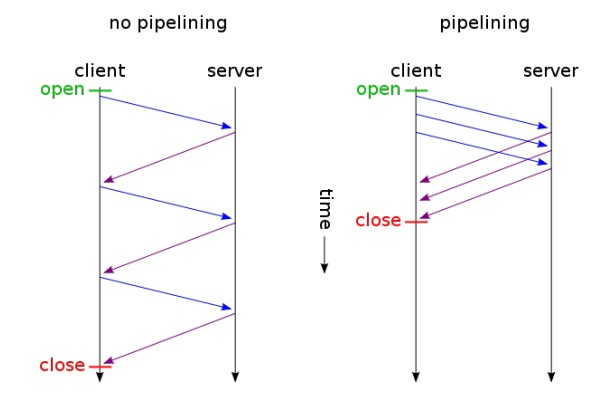
\includegraphics[scale=0.4]{Images/TecnologieWeb/1/Pipelining.jpg}    
\end{center}

\section{Messaggio HTTP}
Il formato generale di un messaggio è il seguente:
\begin{center}
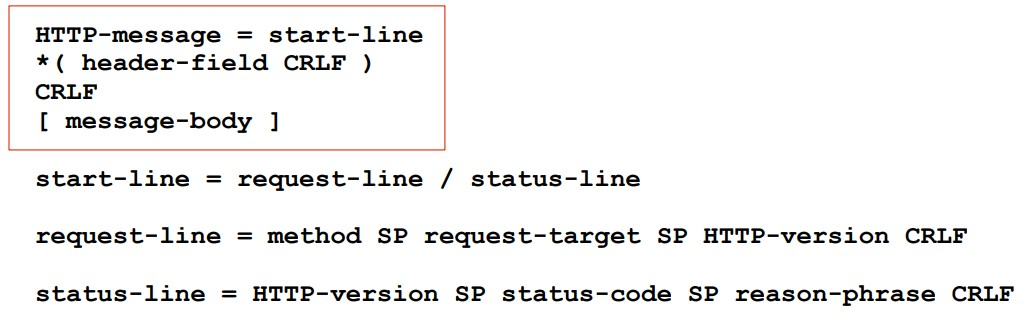
\includegraphics[scale=0.4]{Images/TecnologieWeb/1/MessaggioHTTP.jpg}    
\end{center}

\subsection{Header HTTP}
Gli headers sono in formato MIME e specificano:
\begin{itemize}
    \item caratteristiche generali della trasmissione: data, versione MIME, codifica usata, metodo di caching richiesto o suggerito, connessione, eventuali proxy
    \item caratteristiche della risorsa trasmessa: tipo, lunghezza, codifica, lingua, locazione, range del contenuto, scadenza e data ultima modifica
    \item caratteristiche richiesta
    \item caratteristiche risposta
\end{itemize}

\subsection{Messaggio di HTTP request}
\begin{center}
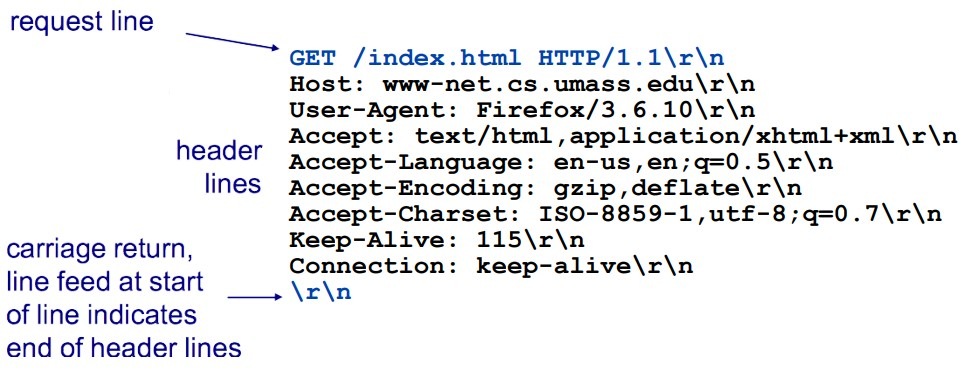
\includegraphics[scale=0.4]{Images/TecnologieWeb/1/HTTPREquestMessage.jpg}    
\end{center}

\section{Metodi}
\begin{center}
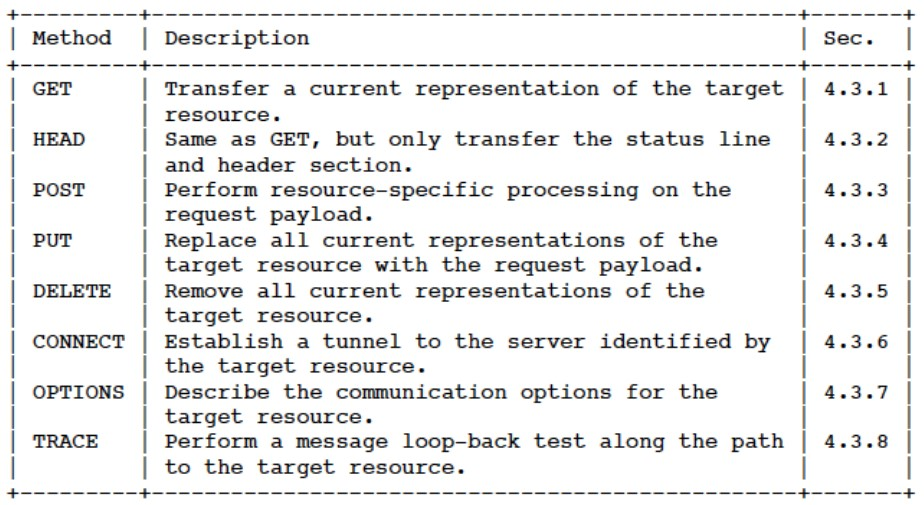
\includegraphics[scale=0.4]{Images/TecnologieWeb/1/MethodsHTTP.jpg}    
\end{center}

\subsection{Metodi HTTP idempotenti e sicuri/non sicuri}
Un metodo \textbf{idempotente} è un metodo HTTP che può essere chiamato molteplici volte senza risultati diversi, la risposta è la medesima indipendentemente da quante volte viene chiamato. Solo i metodi idempotenti possono essere usati per le pipeline.\\
Un metodo \textbf{sicuro} è un metodo HTTP che non modifica le risorse. Ad esempio, usando un metodo GET o HEAD su un URI di una risorsa, non dovrebbe mai modificare quella risorsa.
\hfill \break
Classificazione dei metodi:
\begin{itemize}
    \item GET: sia sicuro che idempotente, è usato per richiedere una risorsa. Una rappresentazione della risorse è ritornata nel messaggio di risposta
    \item POST: nè sicuro nè idempotente, è usato per creare /aggiornare una risorsa (in particolare, risorse subordinate)
    \item PUT: idempotente ma non sicuro, è usato per aggiornare/creare una risorsa
\end{itemize}
La differenza tra POST e PUT è che le richieste di PUT sono idempotenti. Cioè, chiamare lo stessa richiesta di PUT più volte produce sempre lo stesso risultato. Diversamente, chiamare una richiesta POST più volte ha la conseguenza di creare la risorsa più volte.  
\hfill \break
Creazione di una risorsa: POST a una collezione di risorse $\rightarrow$ è compito del server associare la nuova risorsa con la sua risorsa padre e assegnare un ID (l'URI della nuova risorsa).\'E buona pratica ritornare un messaggio di status "201 Created" e la locazione della nuova risorsa creata, dal momento che era incognita fino al momento dell'invio. Questo permette al client di accedervi successivamente, se ne ha bisogno.

\begin{flushleft}
\hspace{1cm}HTTP/1.1 POST /accounts\\
\hspace{1cm}\{\\
\hspace{2cm}\dots\\
\hspace{1cm}\}\\
\end{flushleft}
Risposta:

\begin{flushleft}
201 Created\\
Location: https://api.stormpath.com/accounts/abcdef1234
\end{flushleft}

Creazione di una risorsa: il metodo PUT permette al client di specificare l'identificativo della risorsa da creare
\begin{flushleft}
\hspace{1cm}HTTP/1.1 PUT /accounts/abcdef1234\\
\hspace{1cm}\{\\
\hspace{2cm}"givenName":"John";\\
\hspace{2cm}"surname":"Smith";\\
\hspace{2cm}"status":"Enabled";\\
\hspace{1cm}\}\\
\end{flushleft}


Per aggiornare una risorsa: il metodo POST permette al client di mandare tutti i valori disponibili o anche solo una parte:
\begin{flushleft}
\hspace{1cm}HTTP/1.1 POST /accounts/abcdef1234\\
\hspace{1cm}\{\\
\hspace{2cm}"status":"Enabled";\\
\hspace{1cm}\}\\
\end{flushleft}
In questo caso è meglio usare il metodo PATCH se supportato dal server. Con il metodo PUT ci deve essere l'aggiornamento della intera risorsa e quindi il client deve mandare tutti i valori di attributi per garantire l'idempotenza. 
\begin{flushleft}
\hspace{1cm}HTTP/1.1 PUT /accounts/abcdef1234\\
\hspace{1cm}\{\\
\hspace{2cm}"givenName":"J";\\
\hspace{2cm}"surname":"Smith";\\
\hspace{2cm}"status":"Enabled";\\
\hspace{1cm}\}\\
\end{flushleft}

Generalmente nella pratica si usano sempre POST per la creazione delle risorse e PUT per l'aggiornamento.\\
Oltre a quelli visti in precedenza si hanno anche i seguenti metodi aggiuntivi:
\begin{itemize}
    \item DELETE: idempotente ma non sicuro, cancella la risorsa specificata
    \item HEAD: sia sicuro che idempotente, è simile al metodo GET ma il server deve rispondere solo con l'header, non il body del messaggio. \'E usato per verificare la validità, l'accessibilità e la coerenzad di cache di un URI
\end{itemize}

\subsection{Caratteristiche di un header HTTP di un messaggio di request}
\begin{itemize}
    \item \textbf{From}: indirizzo mail del richiedente, richiede un accordo con l'utente quindi nessuno usa questo campo dell'header
    \item \textbf{Range}: range in bytes della richiesta, usato per riprendere i download
    \item \textbf{Accept, Accept-Charset, Accept-Encoding, Accept-Language}: negoziazione del formato, il cliente specifica cosa è in grado di accettare e il server trova la migliore soluzione
    \item \textbf{If-Modified-Since, If-Unmodified-Since}: usato per richieste condizionali
    \item \textbf{Authorization, Proxy-Authorization}
\end{itemize}

\subsection{Conditional GET}
L'obiettivo è quello di non mandare rappresentazioni di risorse se il cliente dispone già della versione più aggiornata nella cache in modo da non avere ritardi dovuti alla trasmissione e da evitare di usare la connessione. \\ 
Il client specifica la data della versione salvata in cache in una richiesta HTTP \textbf{If-Modified-Since: $<$date$>$} e la risposta del server non contiene nessuna rappresentazione della risorsa se la versione in cache è più aggiornata \textbf{HTTP/1.0 304 Not Modified}.

\begin{center}
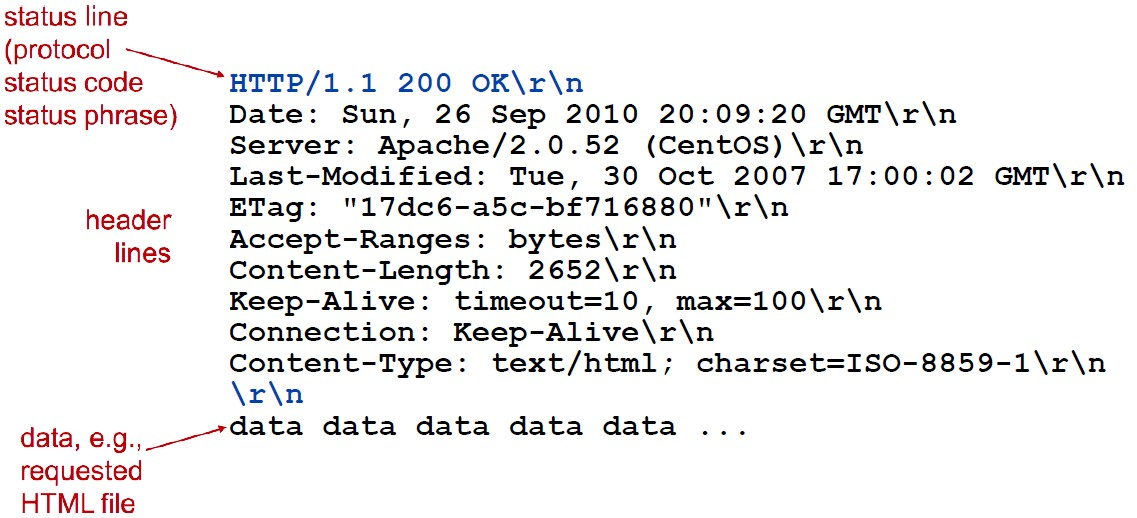
\includegraphics[scale=0.4]{Images/TecnologieWeb/1/MessaggioRispostaHTTP.jpg}    
\end{center}

\subsection{Status Code}
Gli status code appaiono nella prima riga in ogni messaggio dal server al client. \'E formato da 3 cifre: la prima per la classe, le altre due per la specifica richiesta. 
\begin{itemize}
    \item \textbf{1xx $-$ Informational}: risposta temporanea, mentre la richiesta viene gestita
    \item \textbf{2xx $-$ Successful}: il server ha ricevuto, capito e accettato la richiesta
    \item \textbf{3xx $-$ Redirection}: il server ha ricevuto e capito la richiesta ma sono necessarie più azioni da parte del client per soddisfare la richiesta
    \item \textbf{4xx $-$ Client error}: errore di sintassi o richiesta non autorizzata
    \item \textbf{5xx $-$ Server error}: il server non è in grado di soddisfare la richiesta
\end{itemize}

Nelle diapo vengono fatti vedere gli status code più usati.


\subsection{Caratteristiche di un header HTTP di un messaggio di response}
\begin{itemize}
    \item \textbf{Server}: una stringa che descrive il server (tipo, versione, SO)
    \item \textbf{WWW-Authenticate}: contiene una challenge (cioè un codice speciale) per il client, nel caso di status code 401 (unauthorized), il client userà la challenge per generare un codice di autorizzazione per la prossima richiesta
    \item \textbf{Accept-Ranges}: specifica i tipi di ranges che possono essere accettati (bytes o nessuno)
\end{itemize}


\section{Cookies}
Molti siti web usano i cookies. Essi hanno 4 componenti: 
\begin{enumerate}
    \item la riga di inizio del cookie del primo messaggio di risposta HTTP
    \item la riga di inizio dei prossimi messaggi di richieste HTTP
    \item file cookie tenuto nell'host utente, gestito dal suo browser
    \item un database back-end nel sito web
\end{enumerate}

I cookie possono essere usati per: autorizzazioni, carrelli di store online, raccomandazioni, stato della sessione utente (web e-mail).

\begin{center}
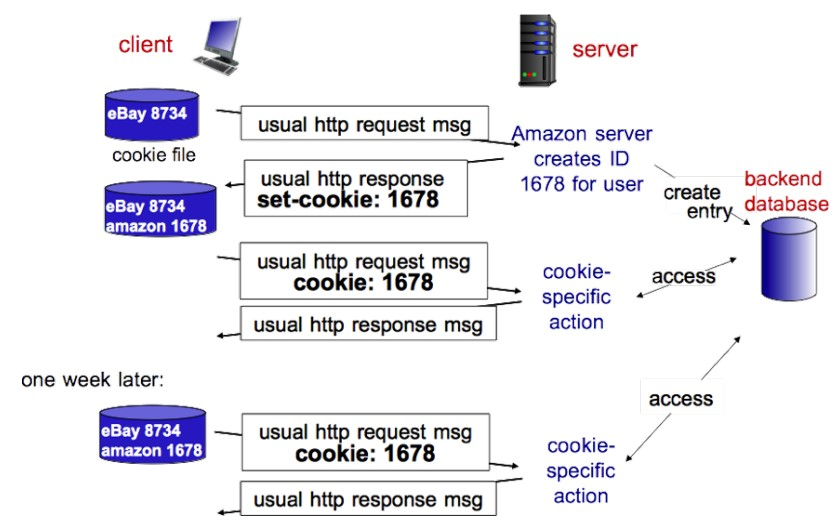
\includegraphics[scale=0.4]{Images/TecnologieWeb/1/Cookies.jpg}    
\end{center}

\section{Proxy}
Un proxy è un'applicazione intermediaria avente sia le funzionalità del client che del server. Un \textbf{proxy trasparente} è un proxy che non modifica le richieste o le risposte aldilà di ciò che gli è necessario per la autenticazione e la identificazione. Mentre un \textbf{proxy non trasparente} modifica le richieste e le risposte in modo tale da fornire servizi aggiuntivi.

\section{Web caching}
Si usa un server proxy per soddisfare le richieste del client senza coinvolgere il server. L'utente dice l'indirizzo del proxy al browser per abilitare l'accesso web con controllo della cache. Il browser manda tutte le richieste HTTP al proxy:
\begin{itemize}
    \item se la rappresentazione delle risorse richieste è nella cache, allora il proxy le ritorna
    \item altrimenti il proxy manda la richiesta all'origin server e poi le manda al client
\end{itemize}

Il proxy si comporta da server per il client che genera la richiesta iniziale, sia da client per l'origin server. Tipicamente le caches sono installate dagli ISP (università, aziende, ISP residenziali). Conviene usare il web caching perchè riduce il tempo di risposta per le richieste, riduce il traffico e permette ai fornitori di contenuti "lenti" di consegnare contenuto in modo effettivo. 


\chapter{Apache HTTP Server}

\section{Architettura}
\begin{center}
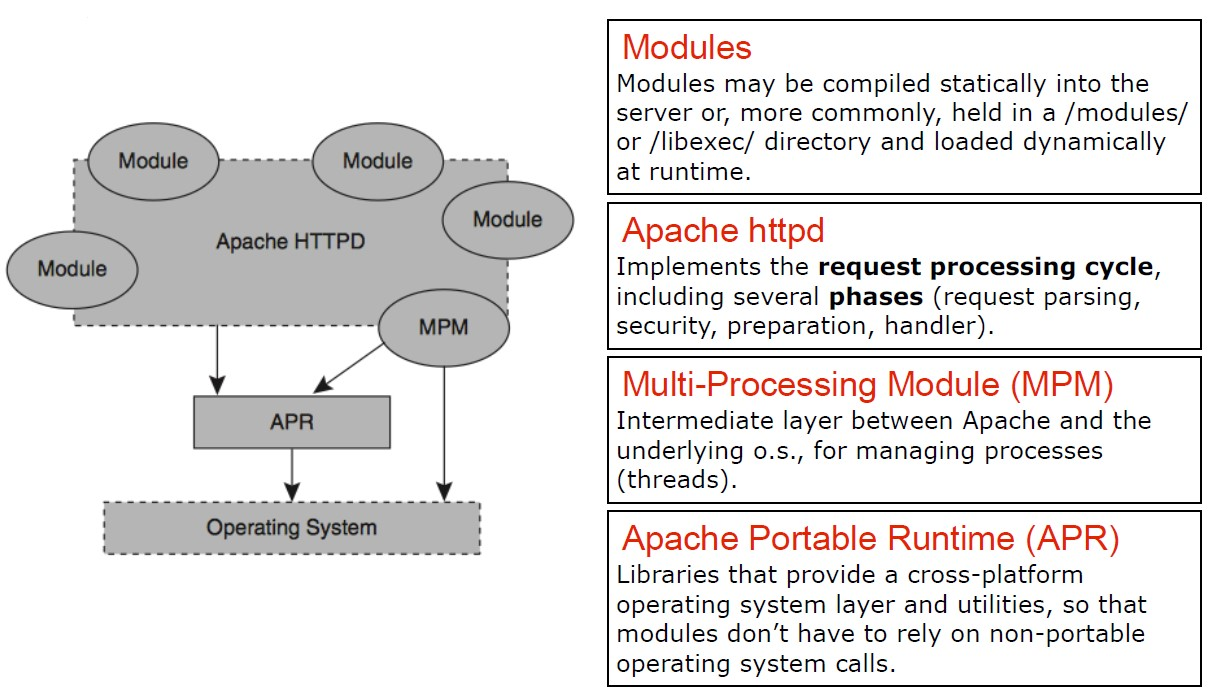
\includegraphics[scale=0.4]{Images/TecnologieWeb/2/Architettura.jpg}    
\end{center}

\section{Multi-processing / multi-threading}
Apache 2.x usa un processo (o thread, in base alla configurazione) per connessione, con I/O bloccante. Il server viene fornito con una selezione di \textbf{Multi-Processing Modules (MPMs)}  che sono responsabili del collegamento alle porte di rete sul macchina, accettando richieste e inviando i processi figli a gestire le richieste.\\
Benefici:
\begin{itemize}
    \item Apache httpd può in modo più efficiente e pulito supportare una grande varietà di sistemi operativi. In particolare, la versione windows del server è ora molto più efficiente, dal momento che mpm winnt può usare le funzionalità di netoworking nativo al posto dello strato POSIX usato nell'Apache httpd 1.3
    \item Il server può essere modificato meglio per le esigenze del sito. Per esempio dei siti che necessitano di grande scalabilità possono scegliere un mpm threaded come worker o event, mentre siti che richiedono stabilità o compatibilità con software precedenti possono usare una prefork.
\end{itemize}

\section{Compilazione e installazione}
\begin{center}
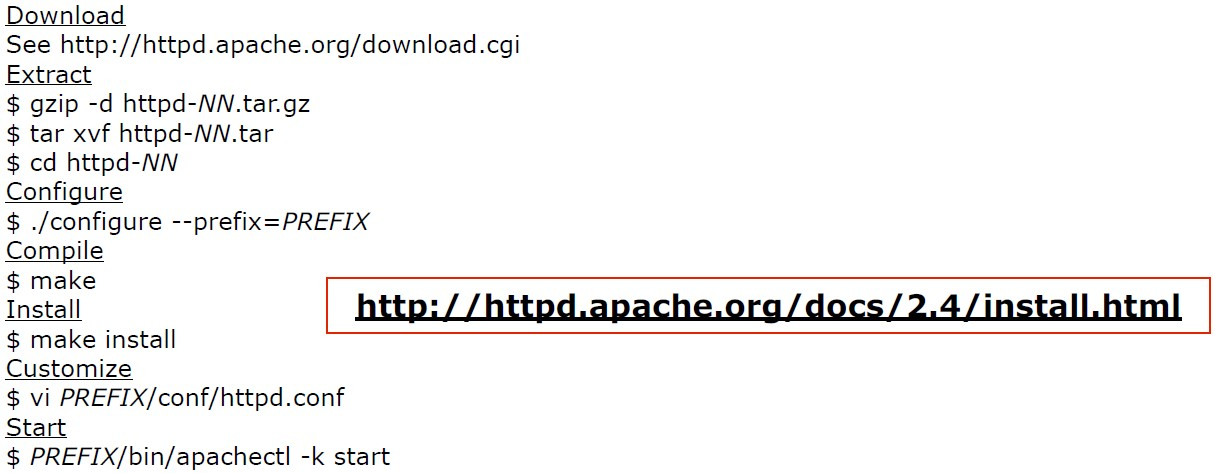
\includegraphics[scale=0.4]{Images/TecnologieWeb/2/CompilazioneInstallazione.jpg}    
\end{center}

\emph{NN} deve essere sostituito con il numero di versione corrente, e \emph{PREFIX} deve essere sostituito con il path del filesystem sotto il quale il server dovrebbe essere installato. Se non viene specificato, quello di default è /usr/local/apache2.

\subsection{File di configurazione e direttive}
Il server HTTP Apache è configurato tramite \textbf{semplici file di testo}. Questi file possono essere posizionati in qualunque varietà di posti, in base a come è stato installato il server. La posizione di default del file di configurazione è \textbf{/usr/local/apache2/conf} e la configurazione di default è chiamata \textbf{httpd.conf}. \\
La configurazione viene frequentemente rotta in molteplici file più piccoli, per facilitare la gestione, che vengono caricati tramite la \textbf{Include directive}. 
Il server è configurato mettendo le \textbf{configuration directives} in quei file di configurazione. Una directive è una keyword seguita da uno o più argomenti che settano il suo valore. \\

Layout di default di Apache httpd 2.4:
\begin{center}
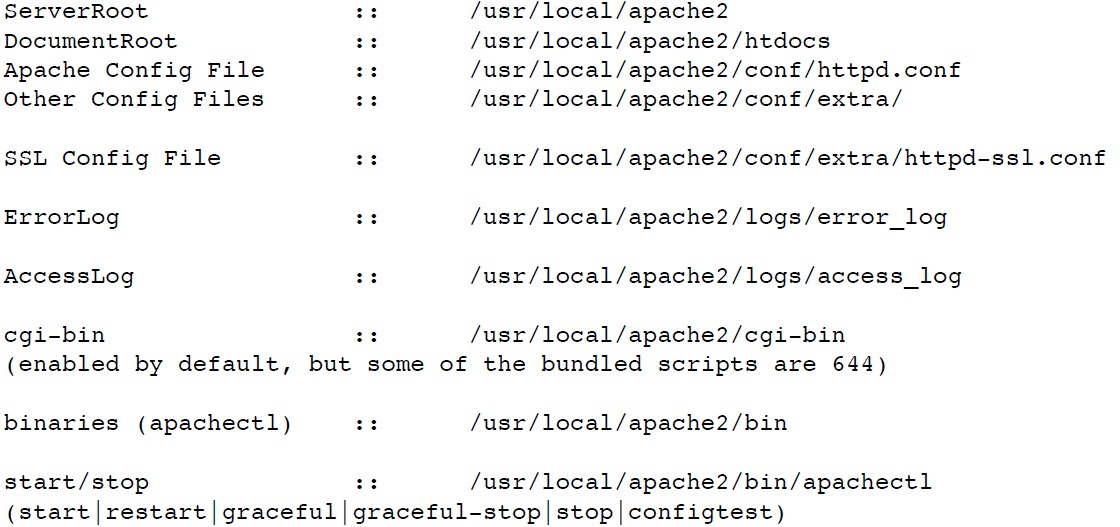
\includegraphics[scale=0.4]{Images/TecnologieWeb/2/FileConfigurazioneCartelle.jpg}    
\end{center}

Configurazione minima:
\begin{center}
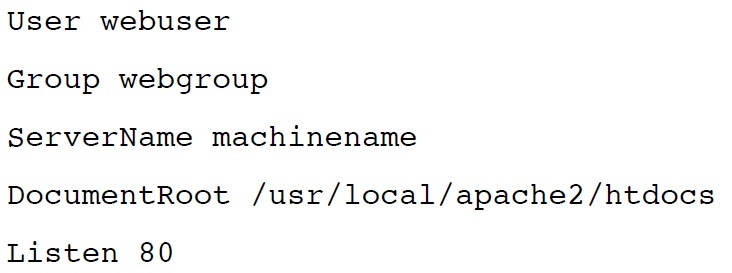
\includegraphics[scale=0.4]{Images/TecnologieWeb/2/ConfigurazioneMinima.jpg}    
\end{center}

\section{Direttiva User}
La direttiva User setta l'ID dell'utente col quale il server risponderà alle richieste. \\
\begin{center}
    \textbf{Sintassi}: \\
User \emph{unix-userid} \\
\end{center}
Dove  \emph{unix-userid} può essere:
\begin{itemize}
    \item un username e quindi ci si riferisce a un certo utente dal suo nome
    \item "\#" seguito da un numero utente quindi ci si riferisce a un utente tramite il suo numero 
\end{itemize}
L'utente non dovrebbe avere privilegi che gli permettono di accedere a file che non dovrebbero essere visibili dall'esterno e nemmeno di eseguire codice che non è connesso a richieste HTTP.

\section{Direttiva Group}
La direttiva Group setta il gruppo sotto al quale il server risponderà alle richieste. Per usare questa direttiva il server deve essere eseguito inizialmente come root. Se si avvia il server come un utente non$-$root, non riuscirà a cambiare al gruppo specificato e continuerà ad eseguire con il gruppo dell'utente originale.  \\
\begin{center}
    \textbf{Sintassi}: \\
Group \emph{unix-group} \\
\end{center}
Dove  \emph{unix-group} può essere:
\begin{itemize}
    \item un nome di un gruppo e quindi ci si riferisce a un certo gruppo dal suo nome
    \item "\#" seguito da un numero di gruppo quindi ci si riferisce a un gruppo tramite il suo numero 
\end{itemize}
\'E consigliato settare un nuovo gruppo specificatamente per il server in esecuzione.

\section{Direttiva ServerName}
La direttiva ServerName setta lo schema di richiesta, hostname e la porta che il server usa per identificarsi.
\begin{center}
    \textbf{Sintassi}: \\
ServerName [\emph{scheme}://]\emph{fully-qualified-domain-name}[:\emph{port}]
\end{center}
Quando si usa \textbf{name-based virtual hosts}, il ServerName in una sezione $<$VirtualHost$>$ specifica quale hostname deve apparire nell'host di richiesta: header per accoppiare questo virtual host.


\subsection{Hostnames e DNS}
Per collegarsi a un server, il client prima deve tradurre l'hostname in un indirizzo IP ovvero la locazione in internet dove il server risiede. Quindi, per avere il server web raggiungibile, è necessario che l'hostname sia nel \textbf{Domain Name System (DNS)}. \\
Gli \textbf{IP-based virtual hosts} usano l'indirizzo IP della connessione per determinare il corretto virtual host da servire per cui si avrò bisogno di un IP separato per ogni host.\\
Con il \textbf{name-based virtual hosting}, il server si affida al client per segnalare l'hostname come parte degli headers HTTP. Usando questa tecnica, molti host diversi possono condividere lo stesso indirizzo IP. 

\subsection{Virtual Hosts}
\textbf{IP-based Virtual Hosts} (un indirizzo IP per ogni sito web)
\begin{center}
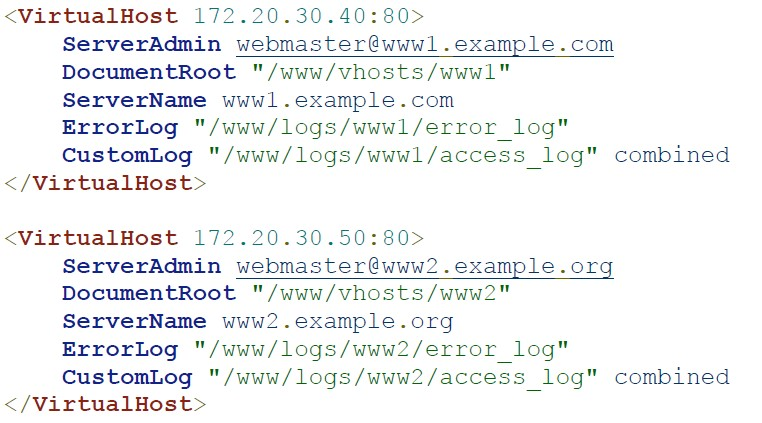
\includegraphics[scale=0.4]{Images/TecnologieWeb/2/VirtualHost.jpg}   
\end{center}
\textbf{Name-based Virtual Hosts} (più di un sito web per ogni indirizzo IP)
\begin{center}
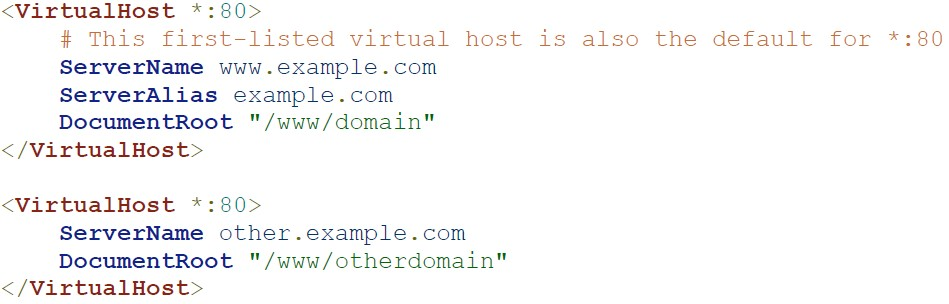
\includegraphics[scale=0.4]{Images/TecnologieWeb/2/VirtualHosts.jpg}  
\end{center}

\section{Direttiva DocumentRoot}
Questa direttiva setta la cartella dalla quale Apache httpd servirà file. Salvo che sia accoppiata con una direttiva come \textbf{Alias}, il server appende il path dall'URL richiesto al document root per creare il path al documento. \\
\begin{center}
    \textbf{Sintassi:}\\
    DocumentRoot \emph{directory-path}\\
\end{center}
Esempio: DocumentRoot "/usr/web"
Successivamente un accesso a http://my.example.com/index.html si riferisce a /usr/web/index.html. Se il \emph{directory-path} non è assoluto allora si assume che faccia riferimento alla \textbf{direttiva ServerRoot}, che setta la cartella nella quale il server vive. 

\section{Direttiva Listen}
La direttiva Listen istruisce Apache httpd ad accettare le richieste in ingresso sulle specifiche porte o combinazioni di porte e indirizzi. \'E una direttiva necessaria. Se non è nel file config, il server non riuscirà ad accendersi.\\
\begin{center}
    \textbf{Sintassi:}\\
    Listen [\emph{IP-address:}]\emph{portnumber}[\emph{protocol}]\\
\end{center}
Molteplici direttive Listen possono essere usate per specificare un numero di indirizzi e porte su cui ascoltare. Ad esempio, per accettare connessioni sia sulla porta 80 che 8000, su tutte le interfacce, si usa:\\
Listen 80\\
Listen 8000\\
Per fare in modo che il server accetti connessioni sulla porta 80 su una interfaccia e sulla porta 8000 su un'altra interfaccia, si usa:
Listen 192.170.2.1:80
Listen 192.170.2.5:8000
Se si usano gli indirizzi IPv6, devono essere messi tra parentesi quadre.


\section{Direttiva ErrorLog}
Per un amministratore di Server Apache HTTP, le migliori risorse sono i log files, specialmente l'error log.

La locazione dell'error log è definita da questa direttiva, che può essere settata globalmente o per host virtuale. Le voci nell'error log dicono all'amministratore cosa quando è andato storto. Spesso dicono anche come risolvere ciò che non è andato giusto. \\
\begin{center}
    \textbf{Sintassi:}\\
    ErrorLog \emph{file-path}$|$syslog[:\emph{facility}]\\
\end{center}
Ciascun messaggio di registro degli errori contiene un codice di errore. L'amministratore può anche configurare il suo error
log per contenere un ID di registro che può quindi correlare a una voce del registro di accesso, per determinare
quale richiesta ha causato la condizione di errore.

\section{Direttiva CustomLog}
Questa direttiva è usata per loggare le richieste al server. Un formato di log è specificato e il logging può opzionalmente reso condizionale in base alle caratteristiche delle richieste usando variabili di ambiente.
\begin{center}
    \textbf{Sintassi:}\\
    CustomLog \emph{file}$|$\emph{pipe format}$|$\emph{nickname} [env$=$[!]\emph{environment-variable}| expr$=$expression]\\
\end{center}
Il primo argomento, che specifica la locazione nella quale il log verranno scritti, può assumere uno dei seguenti valori:
\begin{itemize}
    \item \emph{file}: un filename, relativo al ServerRoot
    \item \emph{pipe}: il carattere di pipe "$|$", seguito dal percorso di un programma per ricevere le informazioni di log sul suo standard input
\end{itemize}
Il secondo argomento specifica cosa verrà scritto sul log. Può specificare sia un nickname definito precedentemente dalla \textbf{direttiva LogFormat} o può essere una stringa esplicita \emph{format}. 
Il terzo argomento è opzionale e controlla se loggare una particolare richiesta o meno.


\section{Direttiva Include}
Questa direttiva permette inclusioni di altri file di configurazione dall'interno del server. 
\begin{center}
    \textbf{Sintassi:}\\
    Include \emph{file-path}$|$\emph{directory-path}$|$\emph{wildcard}
\end{center}
I caratteri speciali in stile shell (fnmatch()) possono essere utilizzati nel nome del file o nelle parti della directory di
il percorso per includere più file contemporaneamente, in ordine alfabetico. Tuttavia, includere l'intera
directory non è raccomandato, perché è facile lasciare accidentalmente file temporanei in un
directory che può causare il fallimento di httpd. Utilizzare invece la sintassi con caratteri speciali mostrata di seguito.
La direttiva Include \textbf{fallirà con un errore} se un'espressione con caratteri speciali non corrisponde a nessun
file. La \textbf{direttiva IncludeOptional} può essere utilizzata se i caratteri speciali non corrispondenti devono essere
ignorati.\\
Il percorso del file può essere assoluto o relativo alla cartella \textbf{ServerRoot}.\vspace{0.2cm}\\
Include /usr/local/apache2/conf/ssl.conf\\
Include /usr/local/apache2/conf/vhosts/*.conf\\
Include conf/vhosts/*/*.conf\\
IncludeOptional conf/vhosts/*/*.conf\\

\section{Direttiva LoadModule}
La direttiva LoadModule si collega al file oggetto o la libreria \emph{filename} e aggiunge la struttura di modulo chiamata \emph{module}$|$ alla lista dei moduli attivi. 
\begin{center}
    \textbf{Sintassi:}\\
    LoadModulo \emph{module filename}
\end{center}
\emph{module} è il nome della variabile esterna di tipo modulo nel file ed è elencata come il \textbf{Module Indentifier} nella documentazione del modulo. Esempio: \vspace{0.1cm}\\
LoadModule status\_module modules/mod\_status.so \vspace{0.1cm}\\
carica il modulo dalla sottocartella modules di ServerRoot.

\section{Direttiva IfModule}
La sezione $<$IfModule \emph{test}$>$ \dots $<$/IfModule$>$ è usata per definire le direttive che sono condizionali sulla presenza di un modulo specifico. Le direttive in una sezione $<$/IfModule$>$ sono elaborate solo se il \emph{test} è vero. Altrimenti tutto ciò che è all'interno delle freccette è ignorato.\\
\begin{center}
    \textbf{Sintassi:}\\
    $<$IfModule [!]\emph{module-file}$|$module-identifier$>$ \dots $<$/IfModule$>$ 
\end{center}
Il \emph{test} nella direttiva di sezione $<$/IfModule$>$ può essere in una tra le seguenti due forme:
\begin{itemize}
    \item \emph{module}
    \item \emph{!module}
\end{itemize}
Nel primo caso, le direttive tra i marker di inizio e di fine vengono elaborate solo se il modulo denominato module è incluso in Apache httpd -- compilato in o dinamicamente
caricato utilizzando LoadModule.
Il secondo formato inverte il test ed elabora le direttive solo se module non lo è incluso

\section{Configurazioni "Local"}
Per applicare direttive a parti specifiche del server:
\begin{center}
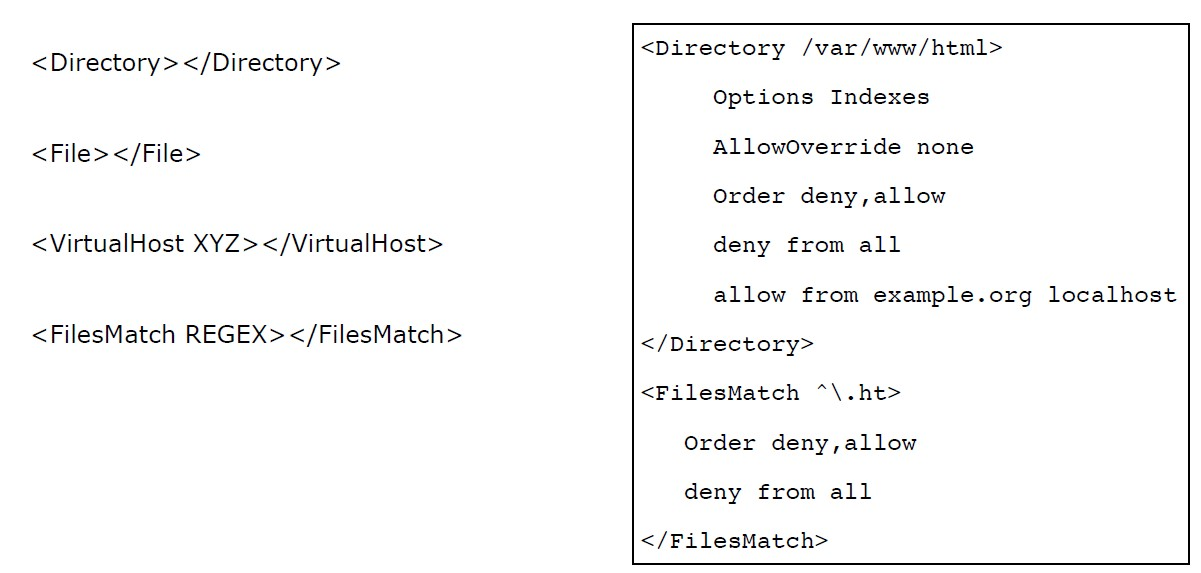
\includegraphics[scale=0.4]{Images/TecnologieWeb/2/ConfigurazioneLocale.jpg}  
\end{center}


\section{Direttiva Options}
La direttiva Options controlla quali funzioni del server sono disponibili in una certa cartella. \\
\begin{center}
    \textbf{Sintassi:}\\
    Options [$+ | -$] \emph{option} [[$+ | -$] \emph{option}] \dots
\end{center}
\emph{option} può essere settato to None, nel caso nessuna delle extra funzionalità è attiva, o una o più delle seguenti:
\begin{itemize}
    \item \textbf{All}: tutte le opzioni eccetto per MultiViews
    \item \textbf{ExecCGI}: l'esecuzione degli script CGI usando \textbf{mod\_cgi} è permessa
    \item \textbf{FollowSymLinks}: Il server seguirà collegamenti simbolici in questa cartella. Questa è l'impostazione predefinita
    \item \textbf{SymLinksIfOwnerMatch}: Il server seguirà solo i link simbolici per i quali il target file (o cartella) è posseduta dallo stesso id utente del collegamento. 
    \item \textbf{Includes}: includes lato server fornito da \textbf{mod\_include} sono permessi
\end{itemize}

\section{.htaccess files}
I file .htaccess \textbf{forniscono un modo per fare cambi di configurazioni su una base per-directory}. 
Un file, contenente una o più direttive di configurazione, è messo in una particolare directory del documento, e le direttive si applicano a quella particolare directory (e tutte le sue sottodir).

È meglio evitare di utilizzare completamente i file .htaccess, avendo accesso a
File di configurazione del server principale httpd. L'utilizzo di file .htaccess rallenta il
Server HTTP Apache. Qualsiasi direttiva che può essere inclusa in un file .htaccess è meglio impostarla in un blocco \textbf{Directory}, poiché avrà lo stesso effetto
con prestazioni migliori.

\section{Aggiustamento prestazioni}
Apache 2.x è un server web general purpose, progettato per fornire equilibrio tra flessibilità, portabilità e performance. Nonostante non sia stato progettato per ottenere record nei benchmark, è in grado di alte performance in molte situazioni reali. Ci sono alcune opzioni che un amministratore del server può configurare per aggiustare le performance di una installazione Apache.

Il problema hardware più grande è rappresentato dalla \textbf{RAM} in quanto un server web non dovrebbe mai fare swap poichè aumenta la latenza.

\section{Direttiva ErrorDocument}
In caso di problema o errore, Apache httpd può essere configurato per fare una di queste 4 opzioni:
\begin{enumerate}
    \item mandare in output un messaggio di errore predefinito
    \item mandare in output un messaggio personalizzato
    \item reindirizzare internamente a un URL path per gestire il problema/errore
    \item reindirizzare a un URL esterno per gestire il problema/errore
\end{enumerate}


\section{Avviamento del server}
Su Unix, il programma httpd è eseguito come \textbf{deamon} ovvero rimane continuamente in background per gestire le richieste. La \textbf{direttiva Listen} specificata nel file di configurazione è di default di 80, quindi è necessario avere i privilegi di root per avviare apache in modo che di colleghi alla porta privilegiata. 

Una volta che il server è avviato e ha eseguito qualche attività preliminari come aprire i log file, lancerà molti \textbf{processi figli} che ascolteranno e risponderanno alle richieste dei clienti. Il processo principale httpd continua l'esecuzione come utente root, mentre i processi figli hanno meno privilegi.

Lo script di controllo \textbf{apachectl} setta alcune variabili d'ambiente che sono necessarie per il funzionamento di https sotto alcuni sistemi operativi, e poi invoca httpd binary.La prima cosa che httpd fa quando è invocato è di mettere e leggere il file di configurazione \textbf{httpd.conf.} Se va tutto bene, il serversi sconnetterà fal terminare e il command prompt ritornerà quasi immediatamente. Questo indica che il server è on e in esecuzione. \'E poi possibile usare il browser per connettersi al server e vedere la \textbf{test page} nella directory DocumentRoot.









% -----------------------------------------------------------------------------

\chapter{XML}
\section{Introduction}
XML sta per \textbf{EXtensible Markup Language} ed è uno strumento indipendente sia dal software che dall'hardware per contenere informazione. 
Un autore di un documento XML può inventare i tag che vuole dal momento che \textbf{il linguaggio XML non ha tag predefiniti}, al contrario di HMTL.\\

\subsubsection{XML separa i dati dall'HTML}. 
Se si necessità di mostrare dati dinamici in un documento HTML, sarà necessario molto lavoro per modificare l'HTML ogni volta che ci sono dei cambiamenti. Con XML, i dati possono essere memorizzati in file separati. In questo modo si potranno separare i compiti e la struttura sarà più chiara. Con poche righe di javascript è possibile leggere un XML esterno e aggiornare il contenuto dei dati nella pagina web. 

\subsubsection{XML semplifica la memorizzazione dei dati}
I dati XML sono memorizzati con formato file di testo. Questo fornisce una modalità di conservare i dati indipendente dall'hardware e dal software. Questo rende più facile creare dati che possono essere condivisi da applicazioni differenti.

\subsubsection{XML semplifica la condivisione dei dati}
Scambiare dati come XML riduce di molto la complessità del trasferimento perchè i dati possono essere da diverse applicazioni incompatibili.

\subsubsection{XML semplifica i cambiamenti di piattaforma}
Il fatto che i file XML siano in formato di testo, rende più semplice espandere, aggiornare a un nuovo sistema operativo, nuove applicazioni e nuovi browser, senza perdere dati.

\subsubsection{Linguaggi internet scritti in XML}
Molti linguaggi internet sono scritti in XML. Questi sono alcuni esempi:
\begin{itemize}
    \item Scalable Vector Graphics (SVG)
    \item Web Service Description Language (WSDL)
    \item RDF Site Summary (RSS)
\end{itemize}


\section{XML tree}
I documenti XML formano una \textbf{struttura ad albero} che inizia con la radice "root" e si divide in foglie "leaves". 

\begin{center}
    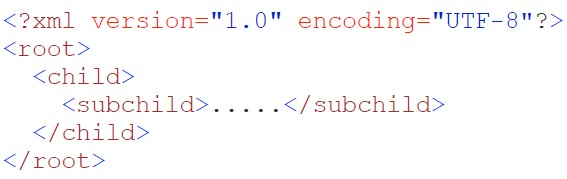
\includegraphics[scale=0.4]{Images/TecnologieWeb/5/Root.jpg}
\end{center}

Il \textbf{prologo (prolog)} definisce la versione di XML. L'albero inizia all'\textbf{elemento root} e si dirama a tutti i livelli. Tutti gli elementi possono avere sottoelementi (\textbf{elementi figli (child)}). I figli sullo stesso livello sono chiamati fratelli \textbf{siglings}. Tutti gli elementi possono avere contenuto e attributi, come HTML.

\begin{center}
    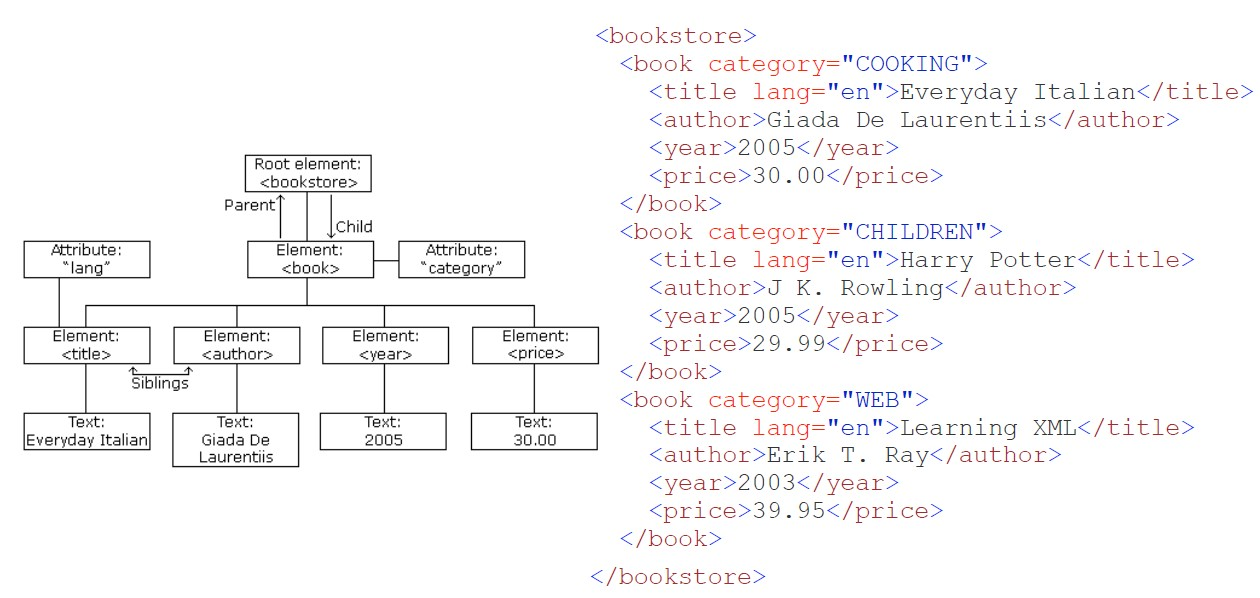
\includegraphics[scale=0.4]{Images/TecnologieWeb/5/ExampleTRee.jpg}
\end{center}

\section{Sintassi XML} 
In XML è \textbf{illegale omettere il tag di chiusura}. Tutti gli elementi devono avere quindi un tag che li chiude. 
\begin{center}
    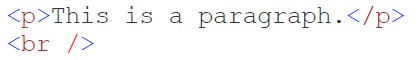
\includegraphics[scale=0.4]{Images/TecnologieWeb/5/Paragrafo.jpg}
\end{center}
\textbf{Eccezione: il prologo} non è parte del documento proprio XML, non ha tag di chiusura. \textbf{I tag XML sono case sensitive}. Ovvero:
\begin{center}
    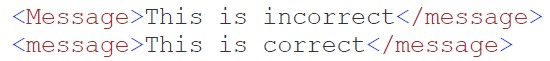
\includegraphics[scale=0.4]{Images/TecnologieWeb/5/Message.jpg}
\end{center}
Tutti gli elementi devono essere annidati correttamente. 

Gli elementi XML possono avere \textbf{attributi} in coppie nome:valore con in HTML e il valore deve essere tra gli apostrofi. 
\begin{center}
    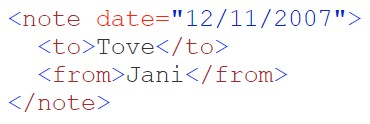
\includegraphics[scale=0.4]{Images/TecnologieWeb/5/NoteDAte.jpg}
\end{center}
La sintassi per scrivere \textbf{commenti} è simile a quelli in HTML, ovvero con i tag "$<!-- $ questo è un commento $-->$". In XML, a differenza di HMTL, gli spazi multipli non vengono compressi in uno unico ma vengono conservati. Alcuni caratteri hanno significato speciale in XML. Ad esempio, questo genererà un errore:
\begin{center}
    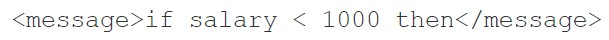
\includegraphics[scale=0.4]{Images/TecnologieWeb/5/MessageIfSalarySbagliat.jpg}
\end{center}
Per evitare questo errore, bisogna sostituire il carattere "$<$" con una \textbf{entity reference}:
\begin{center}
    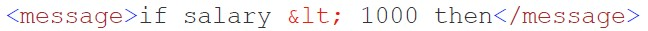
\includegraphics[scale=0.4]{Images/TecnologieWeb/5/MessageIfSalaryGiusto.jpg}
\end{center}
E anche:
\begin{itemize}
    \item \&gt per $>$
    \item \&amp per \&
    \item \&apos per '
    \item \&quot per "
\end{itemize}

\section{Elementi XML}
Un elemento XML è tutto ciò che è compreso tra i suoi tag di apertura e chiusura (compresi). Un elemento può contenere:
\begin{itemize}
    \item altri elementi
    \item testo
    \item attributi
    \item un mix di tutti quelli precedenti
\end{itemize}

Nell'esempio sopra: bookstore e book hanno \textbf{contenuto di elementi} perchè contengono altri elementi. book ha anche un \textbf{attributo} (categoria), title, author, year e price hanno \textbf{contenuto di testo} perchè contengono testo. 
Ci possono essere elementi vuoti:
\begin{center}
    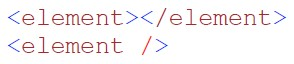
\includegraphics[scale=0.4]{Images/TecnologieWeb/5/Element.jpg}
\end{center}

Gli elementi devono seguire queste \textbf{naming rules}:
\begin{itemize}
    \item Gli elementi sono case sensitive
    \item I nomi degli elementi devono iniziare con una lettera o underscore
    \item I nomi degli elementi non possono iniziare con XML, Xml, XMl, xml, ecc\dots
    \item I nomi degli elementi possono contenere lettere, numeri, underscore, trattini, e frasi
    \item I nomi degli elementi non possono contenere spazi
\end{itemize}

Ogni nome può essere usato, a parte xml. In ogni caso è meglio usare nomi corti e descrittivi, evitando di usare due punti e trattini. Le lettere non inglesi, come le vocali accentate sono accettate in XML ma potrebbero non esserlo dal software usato. 

Consideriamo il seguente esempio:
\begin{center}
    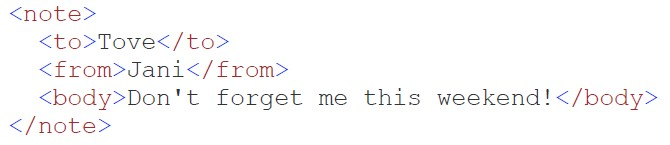
\includegraphics[scale=0.4]{Images/TecnologieWeb/5/NoteTo.jpg}
\end{center}
Immaginiamo che abbiamo creato una applicazione che estrae i tag presenti da quel documento XML per produrre questo output:
\begin{center}
    
\includegraphics[scale=0.4]{Images/TecnologieWeb/5/MessaggioRenderizzato.jpg}
\end{center}
Supponiamo ora, che l'autore del XML abbia aggiunto altre informazioni
\begin{center}
    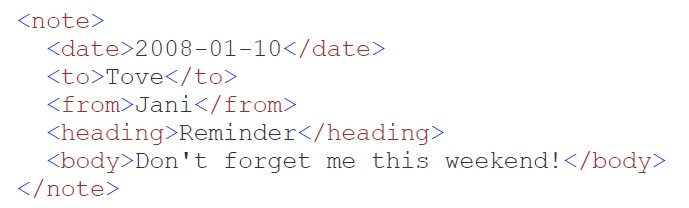
\includegraphics[scale=0.4]{Images/TecnologieWeb/5/NoteDateTo.jpg}
\end{center}
L'applicazione di "rompe" o crasha? L'applicazione dovrebbe essere comunque in grado di trovare i tag degli elementi renderizzati prima e produrre quindi lo stesso output. \textbf{Uno degli aspetto positivi di XML è che può essere esteso senza rompere le applicazioni}.

\section{Attributi XML}
Gli elementi XML possono avere attributi, come HTML, i quali forniscono informazioni aggiuntive. \textbf{Gli attributi spesso forniscono dati che non sono parte dei dati}. Nell'esempio sotto il tipo di file è irrilevante ai dati, ma può essere importante per il software che vuole manipolare l'elemento:
\begin{center}
    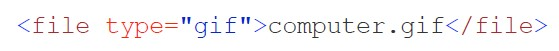
\includegraphics[scale=0.4]{Images/TecnologieWeb/5/File.jpg}
\end{center}
I seguenti esempi sono equivalenti:
\begin{center}
    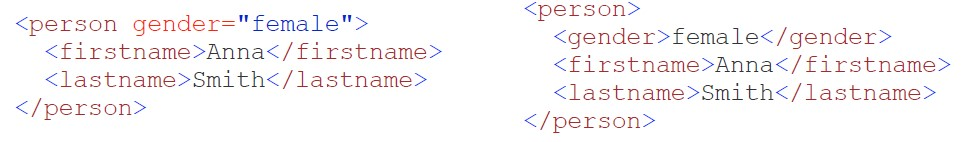
\includegraphics[scale=0.4]{Images/TecnologieWeb/5/Person.jpg}
\end{center}
Non ci sono regole su quando usare attributi e quando elementi. Alcuni \textbf{problemi di quando si usano gli attributi} sono:
\begin{itemize}
    \item gli attributi non possono contenere valori multipli (gli elementi si)
    \item gli attributi non possono contenere strutture ad albero (gli elementi si)
    \item gli attributi non sono facilmente espandibili (per cambiamenti futuri)
\end{itemize}
Gli attributi sono difficili da leggere e mantenere. Usa gli elementi per i dati mentre gli attributi per le informazioni non rilevanti ai dati. 

\section{Namespace XML}
I nomi degli elementi sono definiti dagli sviluppatori. Questo spesso risulta in un conflitto quando si cerca di unire documenti XML da diverse applicazioni.
\begin{center}
    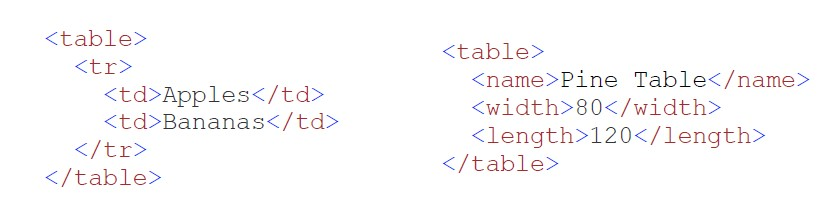
\includegraphics[scale=0.4]{Images/TecnologieWeb/5/Table.jpg}
\end{center}
Se questi fragmenti XML venissero uniti insieme, ci sarebbe un conflitto per i nomi. Entrambi contengono un elemento table, ma gli elementi hanno diverso contenuto e significato. I conflitti di nome possono essere facilmente evitati usando un prefisso:
\begin{center}
    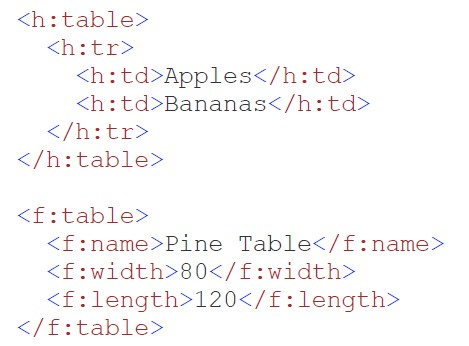
\includegraphics[scale=0.4]{Images/TecnologieWeb/5/TableAliad.jpg}
\end{center}
Quando si usano prefissi in XML, il definito \textbf{namespace} per il prefisso deve essere definito. Il namespace è definito dall'\textbf{attributo xmlns} nel tag iniziale di un elemento.

La dichiarazione di namespace ha la seguente sintassi:\\

xmlns:\emph{prefix} $=$ "URI"
\begin{center}
    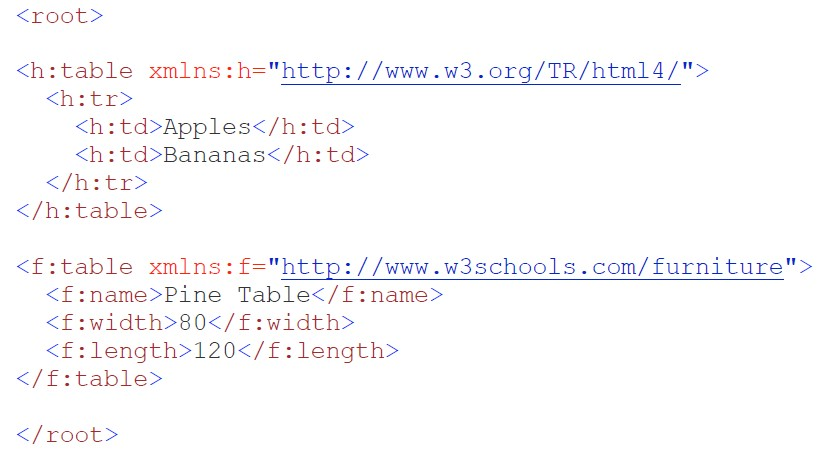
\includegraphics[scale=0.4]{Images/TecnologieWeb/5/furniture.jpg}
\end{center}
Nell'esempio sopra, l'attributo xmlns nel tag table da ai prefissi h: e f: un namespace qualificato. Quando un namespace è definito per un elemento, tutti gli elementi figli con lo stesso prefisso sono associati allo stesso namespace. I namespace possono essere dichiarati in elementi in cui sono usati o nell'elemento root:
\begin{center}
    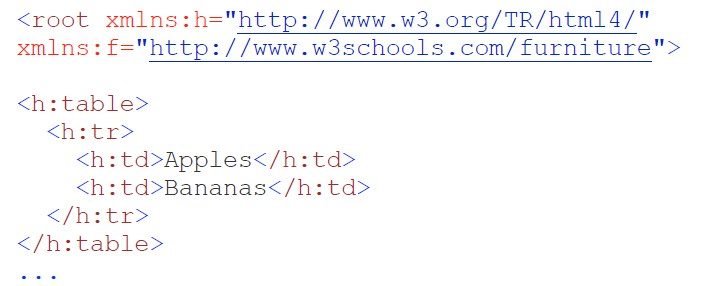
\includegraphics[scale=0.4]{Images/TecnologieWeb/5/xmlns.jpg}
\end{center}

Se definiamo un namespace di default evitiamo poi di dover usare prefissi in tutti gli elementi figli. Ha la seguente sintassi:\\

xmlns $=$ "\emph{namespaceURI}"\\

Per cui, l'esempio precedente potrebbe diventare:

\begin{center}
    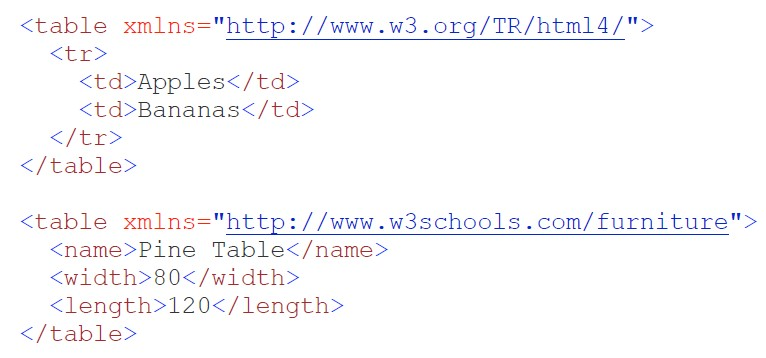
\includegraphics[scale=0.4]{Images/TecnologieWeb/5/TableXlmns.jpg}
\end{center}

\section{Codifca XML}
I documenti XML possono contenere caratteri internazionali, come i norvegesi æøå e i francesi êèé. Usiamo il prologo per specificare la codifica:

\begin{center}
    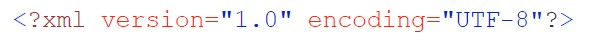
\includegraphics[scale=0.4]{Images/TecnologieWeb/5/xmlversion.jpg}
\end{center}
Dove UTF sta per Unicode Transformation Format. Lo standard XML dice che tutto il software XML capisce sia UTF8 che UTF16 oltre a ISO$-$8859$-$1, Windows$-$1252 e ASCII.

\section{Visualizzazione XML}
I file XML possono essere visti in tutti i principali browser. Ovviamente non bisogna aspettarsi che sia visualizzato come le pagine HTML. 
\begin{center}
    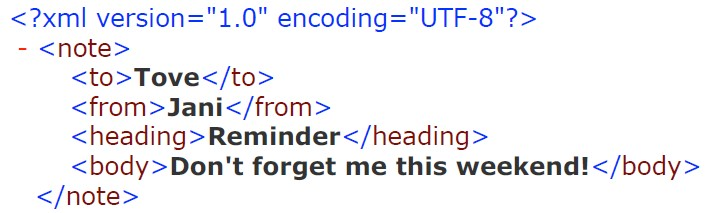
\includegraphics[scale=0.4]{Images/TecnologieWeb/5/Reminder.jpg}
\end{center}
Nota che un documento XML verrà visualizzato con gli elementi radice e figli codificati a colori. Il simbolo $+$ o $-$ dell'elemento indica che si può nascondere il contenuto. 


\section{Tipi di documento XML}
Un documento XML formato con la corretta sintassi è chiamato "Ben formato". Un documento "valido" deve essere anche conforme alla \textbf{document type definition}. Ci sono due diverse document type definition che possono essere usate con XML:
\begin{itemize}
    \item \textbf{DTD} - l'originale Document Type Definition
    \item \textbf{XML Schema} - una alternativa a DTD basata su XML
\end{itemize}
Quando usare un DTD o Schema?
\begin{enumerate}
    \item Gruppi indipendenti di persone possono essere d'accordo per usare uno DTD standard o schema per scambiare i dati
    \item La tua applicazione può usare uno standatd DTD o schema per verificare che i dati che ricevi dall'esterno sono validi
    \item Puoi anche usare un DTD o schema per verificare i tuoi dati
\end{enumerate}

Quando non usare un DTD o schema?
In principio, XML non richiede un DTD o schema. Quando si sta sperimentando con XML o si sta lavorando su piccoli file XML, creare DTD potrebbe essere uno spreco di tempo. Se si sta invece sviluppando applicazioni, aspetta finchè le specifiche sono stabili prima di aggiungere una definizione di documento. Altrimenti il tuo software potrebbe non lavorare più per dei validation errors. 

\subsection{XML DTD}
Una doctype declaration può essere anche usata per definire caratteri speciali e caratteri stringhe, usate nel documento:
\begin{center}
    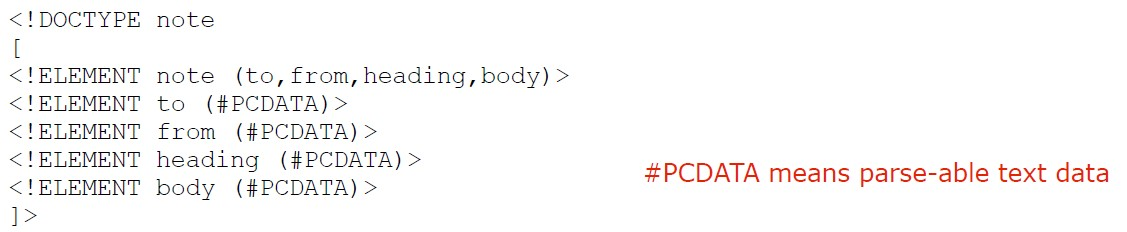
\includegraphics[scale=0.4]{Images/TecnologieWeb/5/DTD.jpg}
\end{center}

\subsection{XML Schema}
XML Schema è una alternativa a DTD basata su XML.
\begin{center}
    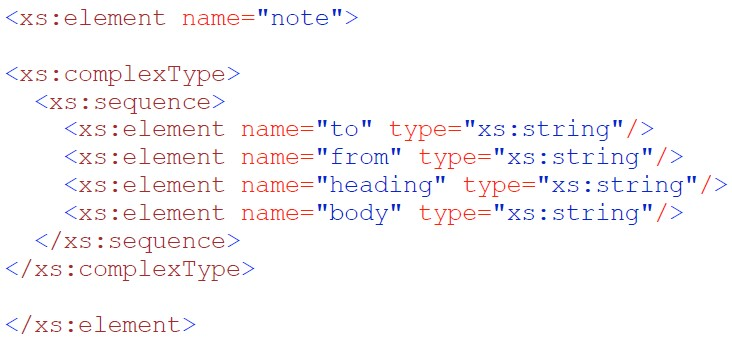
\includegraphics[scale=0.4]{Images/TecnologieWeb/5/Scherma.jpg}
\end{center}
\textbf{Gli XML Schema sono molto più potenti del DTD}:
\begin{itemize}
    \item Gli schemi XML sono scritti in XML
    \item Gli schemi XML sono estensibili ad aggiunte
    \item Gli schemi XML supportano i tipi di dato
    \item Gli schemi XML supportano i namespace
\end{itemize}


%--------------------------------------------------------

\chapter{JSON}
\section{Panoramica}
JSON sta per \textbf{J}ava\textbf{S}cript \textbf{O}bject \textbf{Notation}. \'E una sintassi per memorizzare e scambiare dati. \'E molto leggero e più facile di XML, vedi il confronto sotto.
\begin{center}
    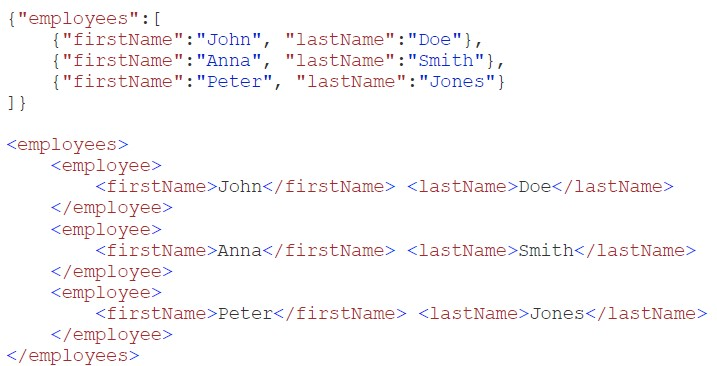
\includegraphics[scale=0.4]{Images/TecnologieWeb/6/employee.jpg}
\end{center}
Il formato JSON è sintatticamente identico al codice per creare oggetti in Javascript.
\begin{center}
    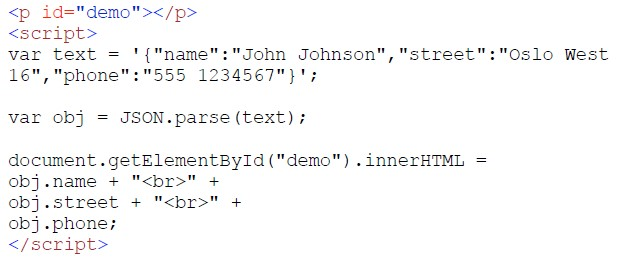
\includegraphics[scale=0.4]{Images/TecnologieWeb/6/script.jpg}
\end{center}
Data questa similarità, invece di usare un parser (come fa XML), un programma javascript  può usare una funzione standard per convertire i dati JSON in oggetti nativi di Javascript. 

Aspetti comuni a XML:
\begin{itemize}
    \item Entrambi sono "self describing" ovvero che sono leggibili e comprensibili normalmente
    \item Entrambi hanno struttura gerarchica
    \item Entrambi possono essere convertiti e usati da molti linguaggi di programmazione
    \item Entrambi possono essere recuperati con un XMLHttpRequest
\end{itemize}

Aspetti diversi da XML:
\begin{itemize}
    \item JSON non usa tag di chiusura
    \item JSON è più breve
    \item JSON è più veloce da leggere e scrivere
    \item JSON può usare array
\end{itemize}

\section{Sintassi}
La sintassi di JSON è derivata dalla sintassi della notazione degli oggetti di Javascript:
\begin{itemize}
    \item I dati sono in coppie nome:valore
    \item I dati sono separati da virgole
    \item Le parentesi graffe delimitano gli oggetti
    \item Le parentesi quadre delimitano gli array
\end{itemize}
Una coppia nome:valore consiste in un campo nome, tra virgolette, seguito da due punti e da il valore.:
\begin{center}
    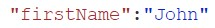
\includegraphics[scale=0.4]{Images/TecnologieWeb/6/FirstNameJohn.jpg}
\end{center}
Un valore JSON può essere:
\begin{itemize}
    \item un numero (intero o floating point)
    \item una stringa (tra virgolette)
    \item un booleano (vero o falso)
    \item un array (tra parentesi quadre)
    \item un oggetto (tra parentesi graffe)
    \item null
\end{itemize}
Gli oggetti JSON sono scritti dentro le parentesi graffe e possono contenere molteplici coppie nome:valore:
\begin{center}
    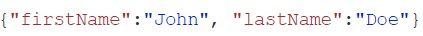
\includegraphics[scale=0.4]{Images/TecnologieWeb/6/FirstLastNAme.jpg}
\end{center}
Gli array JSON possono contenere molteplici oggetti:
\begin{center}
    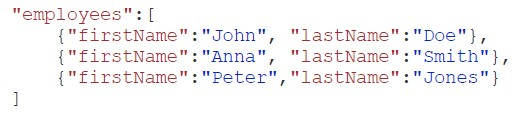
\includegraphics[scale=0.4]{Images/TecnologieWeb/6/Employees.jpg}
\end{center}


%--------------------------------------------

\chapter{Motori di ricerca per il web}
\section{Introduzione}
Molto simile all'\textbf{information retrieval}, che è la parte dell'informatica
che studia il \textbf{recupero di informazioni} da una collezione di
\textbf{documenti scritti}. I documenti recuperati mirano a soddisfare un' \textbf{informazione utente necessaria} tipicamente espressa in \textbf{linguaggio naturale}. Rispetto all'information retrieval, la ricerca web ha proprietà specifiche:
\begin{itemize}
    \item \textbf{Collegamenti} tra pagine web che possono essere sfruttati
    \item \textbf{Collezionare}, memorizzare e \textbf{aggiornare} documenti è più difficile
    \item Di solito, il \textbf{numero di utenti} è molto grande
    \item Lo \textbf{spam} è un problema
\end{itemize}

\section{Eterogeneità dei tipi di documenti}
Alcuni tipi di file che un motore di ricerca dovrebbe essere in grado di elaborare, e quindi trovare: 
\begin{multicols}{2}
\begin{itemize}
    \item application/ms-excel (different versions)
    \item application/mspowerpoint (different versions)
    \item application/msword (different versions)
    \item application/pdf (different versions)
    \item application/postscript
    \item application/x-dvi
    \item application/x-tar
\end{itemize}
\begin{itemize}
    \item application/x-zip-compressed
    \item text/html (different versions and encodings)
    \item text/plain (different encodings)
    \item text/rtf
    \item application/xml
    \item text/xml
    \item \dots
\end{itemize}
\end{multicols}


\section{Eterogeneità delle queries}
Ci sono \textbf{4 principali tipi di query}:
\begin{itemize}
    \item \textbf{Queries informative}: trova informazioni generali riguardo un certo argomenti
    \item \textbf{Queries navigazione}: trova uno specifico sito. Es: "facebook"
    \item \textbf{Queries di transazione}: trova siti che forniscono certi servici. Es: "Adobe Reader download"
    \item \textbf{Queries di connessione}: Trova le pagine connesse. Es: "link:www.unipr.it" trova tutte le pagine che si collegano a http://www.unipr.it
\end{itemize}

\section{Motori di ricerca}
Hanno 3 funzionalità principali:
\begin{itemize}
    \item \textbf{Crawling}: perlustrare internet per un contenuto, guardando il codice per ogni URL che trovano
    \item \textbf{Indexing}: memorizza e organizza il contenuto trovato durante il processo di crawling. Una volta che la pagine è nell'indice verrà poi mostrata come risultato delle query
    \item \textbf{Ranking}: Fornisce i pezzi di contenuto che corrispondono al meglio a ciò che la query richiede. Ciò significa che i risultati sono ordinati dal più al meno rilevante
\end{itemize}

\subsection{Dimensione dell'indice}
Quanto è grande un indice tipico di un motore di ricerca? Questo numero corrisponde al numero di pagine indicizzate

\begin{center}
    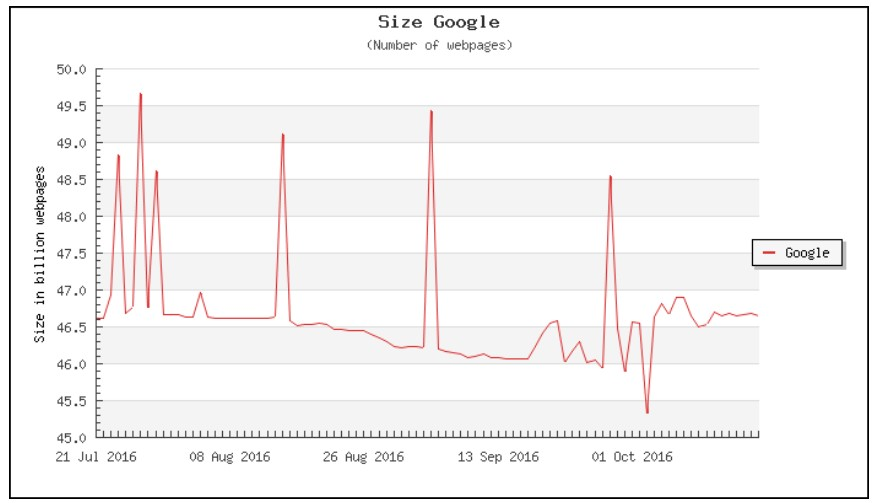
\includegraphics[scale=0.4]{Images/TecnologieWeb/7/IndexSize.jpg}
\end{center}

\subsection{Traffico web e larghezza di banda}
L'indice deve essere periodicamente aggiornato poichè le pagine vengono aggiunte, modificate e rimosse. 

Quanti dati devono essere trasferiti per fare ciò? Alcuni numeri recenti di netcompetition.org dicono chce nella parte americana di internet, google trasferisce circa 60 petabytes al mese. 

\subsection{Scalabilità}
Da un grafico nelle diapo si vede che l'andamento del numero di hostname nel tempo è praticamente esponenziale. Le stime fatte ovviamente sono riferite al \textbf{"surface web"} cioè la parte di web a cui si può accedere dagli attuali web crawler. Anche i migliori crawler attuali non riescono a trovare pagine senza inlinks e tutte le pagine che sono state generate dinamicamente. 

Il termine "\textbf{deep web}" si riferisce a tutte le pagine web che attualmente non sono indicizzate da alcun motore di ricerca. Il deep web si stima sia \textbf{dalle 15 alle 500 volte più grande del surface web}. 

Alcuni tipi di "deep resources":
\begin{itemize}
    \item Contenuto dinamico al quale non si può accedere automaticamente. Ad esempio pagine che sono generate dinamicamente dopo aver compilato un web form.
    \item Contenuti privati o scollegati
    \item Contenuto "scriptato", che richiede l'esecuzione di codice (java, javascript, flash, ecc\dots)
    \item Formati di file strani non gestiti dagli attuali motori di ricerca
\end{itemize}
Il "\textbf{Dark Web}" è un subset del deep web. Per raggiungere il dark web è necessario aderire a specifiche reti di overlay che lo consentano
applicazioni per scambiarsi messaggi con uno pseudonimo e
in modo sicuro ("darknet"), come Tor, I2P e Freenet.


\section{Il grafo del web}
Possiamo vedere il web statico come formato da pagine HTML statiche insieme con gli hyperlink tra loro come un grafo diretto: ogni pagina è un nodo e ogni hyperlink è una freccia direzionale. 

Gli hyperlink entranti una pagina sono chiamati \textbf{inlinks} mentre quelli uscenti sono chiamati \textbf{outlinks}. 

\begin{center}
    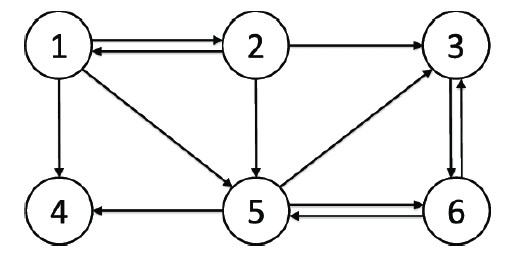
\includegraphics[scale=0.4]{Images/TecnologieWeb/7/Graph.jpg}
\end{center}

Esiste una prova del fatto che quei collegamenti non sono distributi randomicamente. La distribuzione degli inlinks segue una \textbf{legge di potenza} ovvero \textbf{il numero totale di pagine aventi esattamente k inlinks è proporzionale a k}$^{2.1}$.
Inoltre, molti studi hanno suggerito che il grafo del web ha una \textbf{forma a papillon}. 
\begin{center}
    \includegraphics[scale=0.4]{Images/TecnologieWeb/7/BowTie.jpg}
\end{center}
I collegamenti non sono creati randomicamente:
\begin{center}
    \includegraphics[scale=0.4]{Images/TecnologieWeb/7/WebGraph.jpg}
\end{center}

\section{Web crawling}
Un \textbf{crawler di base} (aka robot, bot, spider) consiste di:
\begin{itemize}
    \item Una \textbf{coda} di URI da visitare
    \item Un metodo per \textbf{reperire} le risorse web e elaborare i dati HTTP
    \item Un \textbf{parser di pagina} per estrarre collegamenti dalle risorse recuperate
    \item Una \textbf{connessione} al \textbf{indexer} del motore di ricerca
\end{itemize}

La modalità di base per le operazioni:\\
Inizializza la coda con gli URI di \textbf{seed pages} conosciute e poi ripeti all'infinito:
\begin{enumerate}
    \item Prendi l'URI dalla coda
    \item Recupera e converti la pagina
    \item Estrai gli URI dalla pagina
    \item Aggiungi i nuovi URI alla coda
    \item Manda la pagina all'indexer
\end{enumerate}
Considerando che nel web ci sono circa 60 miliardi di pagine e assumendo di voler fare il crawl di ogni pagina una volta all'anno, significa che bisogna analizzare 1929 pagine al secondo. Da ciò, si nota banalmente, di come sia necessario un crawler \textbf{altamente scalabile}.\\

A parte quelli di scalabilità, ci sono ulteriori problemi: come identificare le pagine spam, come identificare i duplicati di pagine già viste, come evidare le spider traps, come si distribuiscono le macchine necessarie, come gestire la latenza, ecc\dots

\subsection{Robot exclusion standard}
Esclude certe risorse dall'accesso dei robot e quindi, anche dall'indicizzazione dei motori di ricerca. Un file chiamato "robots.txt" nella cartella di dominio top$-$level 
specifica a quali risorse i crawler hanno il permesso di accedere. \textbf{Attenzione}: questo "standard" non è uno standard nel senso tipico, è puramente consultivo. 

\section{Ranking basato sull'analisi dei collegamenti}
Si applicano le idee delle analisi di rete a grafo del web. I link sono raccomandazioni nel senso che se una pagina ha molti inlinks probabilmente è importante. GLi \textbf{anchor text} (testo visibile selezionando un link, etichetta descrittiva) possono essere usati come descrizione dei documenti. 
\begin{itemize}
    \item \textbf{Assunzione 1}: un hyperlink è segnale di qualità o interesse popolare
    \item \textbf{Assunzione 2}: l'anchor text di un link descrive la pagina target
\end{itemize}
Ci sono due algoritmi popolari di ranking: \textbf{PageRank} e \textbf{HITS}.

\subsection{PageRank}
Il metodo per calcolare PageRank e gli elementi connessi sono sotto brevetto. \'E un algoritmo di analisi di collegamenti che produce un ranking delle pagine web che non dipende dalle queries. L'algoritmo è eseguito periodicamente dall'\textbf{indexer}. Il risultato è un \textbf{ranked index}. 

Assumiamo che la pagina \emph{p} sia collegata dalle pagine $q_1, \dots, q_n$. Sia \emph{d} la probabilità che un navigatore randomico si annoi della pagina che sta visitando e si sposti ad un'altra pagina scelta a caso (tipicamente $d=0.85$). Sia \emph{C(p)} il numero di collegamenti da \emph{p}. Il PageRank di \emph{p} è allora:
\[
PR(p) = (1 - d) + d\left[\frac{PR(q_1)}{C(q_1)} + \dots + \frac{PR(q_n)}{C(q_n)}\right]
\]
Le queries dell'utente ottengono un sottoinsieme dell'intero set di pagine, ordinate secondo il Page Rank.\\

\noindent Esempio 1:
\begin{center}
    \includegraphics[scale=0.4]{Images/TecnologieWeb/7/AB.jpg}
\end{center}

\noindent$d = 0.85$\\

\noindent$PR'(A) = (1 - d) + d\dfrac{PR(B)}{C(B)} = (1-d) + dPR(B)$\\
$PR'(B) = (1 - d) + d\dfrac{PR(A)}{C(A)} = (1-d) + dPR(A)$\\

\begin{enumerate}
    \item Ipotesi $PR(A) = PR(B) = 1$ allora $PR'(A) = PR'(B) = 1$ e quindi l'ipotesi era corretta
    \item Ipotesi $PR(A) = PR(B) = 0$ allora $PR'(A) = PR'(B) = 0.15$ e poi $PR'(A) = PR'(B) = 0.2775$ \dots finchè $PR'(A) = PR'(B) = 1$. Converge sempre 
\end{enumerate}\vspace{0.2cm}

\noindent Esempio 2:
\begin{center}
    \includegraphics[scale=0.4]{Images/TecnologieWeb/7/PageRank.jpg}
\end{center}

\noindent$d = 0.85$\\

\noindent$PR'(A) = (1 - d) + d\dfrac{PR(C)}{C(C)}$\vspace{0.1cm}\\
$PR'(B) = (1 - d) + d\dfrac{PR(A)}{C(A)}$\vspace{0.1cm}\\
$PR'(C) = (1 - d) + d\left[\dfrac{PR(A)}{C(A)} + \dfrac{PR(B)}{C(B)} + \dfrac{PR(D)}{C(D)} \right]$\vspace{0.1cm}\\
$PR'(D) = (1 - d) + d\cdot0 = 1 - d$\vspace{0.1cm}\\

Inizia con $PR(x) = 1$ per ogni pagina x poi calcola PR' finchè non converge. Il principale difetto di PageRank è che calcola un solo singolo score per ogni risorsa del web. Una risorsa web potrebbe non essere importante da una vista globale ma molto importante per uno specifico argomento. 

\textbf{Topic-sensitive PageRank} prova a risolvere questo problema:
\begin{itemize}
    \item Definisce un set ti argomenti popolari (calcio, windows, obama)
    \item Usa algoritmi di classificazione per assegnare ad ogni risorsa web a uno o più di quegli argomenti
    \item Per ogni argomento, calcola un topic$-$sensitive PageRank limitando gli spostamenti casuali a pagine dell'algoritmo corrente
    \item Nel momento della query, ne identifica l'argomento e usa il corrispondente score di PageRank 
\end{itemize}

\subsection{HITS}
Kleinberg identifica due tipi di pagina web:
\begin{multicols}{2}
\begin{itemize}
    \item \textbf{Authority}: una pagina che è una fonte autorevole di informazione per la query
    \item \textbf{Hub}: una lista di puntatori a pagine che sono correlate all'argomento della query
\end{itemize}
\begin{center}
    \includegraphics[scale=0.4]{Images/TecnologieWeb/7/HITS.jpg}
\end{center}
\end{multicols}
C'è una relazione di rinforzo mutuo tra due tipi di pagine web: \emph{"good hubs point to good authorities and viceversa"}.\\

\begin{enumerate}
    \item \textbf{Sampling phase}: le parole della query sono usate per costruire un \textbf{root set} di pagine, usando un motore che analizza il contenuto testuale. 
    
    Dopodichè, il root set è esteso in un \textbf{base set}, aggiungendo tutte le pagine che puntano e che sono puntate dalla pagine del root set. Il base set dovrebbe contenere tutte le pagine che si adattano al meglio alla query. 
    
    \item \textbf{Weight-progagation phase}: Il \textbf{peso di un' authority a}$_p$ e il \textbf{peso di un hub h$_p$}, non negativi e inizializzati con valore 1, sono assegnati ad ogni pagina \emph{p} del base set. 
    
    Regola di aggiornamento:
    \begin{itemize}
        \item $a_p$ è la somma dei pesi degli hub delle pagine che puntano a \emph{p}
        \item $h_p$ è la somma dei pesi delle authority delle pagine che sono puntate da \emph{p}
        \item normalizzazione:
        \[
           \dfrac{a_p}{\sum\limits_i \sqrt{a_i}} \hspace{1cm} \dfrac{h_p}{\sum\limits_i \sqrt{h_i}}
        \]
    \end{itemize}
    \'E applicata iterativamente finchè i pesi delle authority e degli hub convergono (procedura molto onerosa).
\end{enumerate}

 Alla fine sono prodotti due ranking: uno degli hub e uno delle authority. Ogni tanto HITS tende a generalizzare o deviare dall'argomento dato, in particolare quando gli hubs coprono più argomenti diversi.
 Una possibile soluzione è quella di comparare le parole nella query con le parole attorno al link, per ottenere una versione pesata della regola di aggiornamento. Un'altra possibilità è quella di frammentare un hub grande in molteplici hublet più piccoli e di ignorare quelli che sono meno correlati all'argomento della query. 
 
 \section{Confronto HITS e PageRank}
 PageRank può essere precalcolato, HITS deve essere calcolato nel momento della query per cui è molto oneroso. Scelte diverse riguardanti il modello formale: HITS modella hub e authority e usa un set del web graph. 
 Potremmo però applicare PageRank ad un sottoinsieme e HITS su tutti il grafo Web.
 
 
 \chapter{JavaScript basics}
 \section{Introduction}
 Javascript è il \textbf{linguaggio di programmazione del web}. La maggior parte dei siti web moderni usa javascript e tutti i moderni browser includono \textbf{interpreti javascript}. Nell'ultima decade, \textbf{Node} ha permesso la programmazione javascript al di fuori dei web browser e il suo successo ha reso javascript il linguaggio di programmazione più usato tra gli sviluppatori.
 
 \section{Model View Controller (MVC}
MVC è un pattern architetturale utilizzato per organizzare parti di codice in 
campi puliti e separati, secondo le responsabilità e
caratteristiche di ciascuno di essi.

Il \textbf{modello} è la rappresentazione dei dati che verranno utilizzati in
l'applicazione; il modello è indipendente dalla View, in quanto esso
non sa come verranno visualizzati i dati. La \textbf{view} è l'interfaccia utente che visualizzerà i contenuti dell'applicazione; la vista è indipendente dal Modello in quanto contiene un mucchio di elementi grafici che possono essere utilizzati in qualsiasi applicazione (ad es. pulsanti, etichette, cursori, ...).
Il \textbf{controller} gestisce come dovrebbero essere i dati nel Modello
visualizzato nella vista; è fortemente dipendente dal Modello e
la vista poiché ha bisogno di sapere quali dati gestirà e quali
elementi grafici con cui dovrà interagire

\begin{center}
    \includegraphics[scale=0.4]{Images/TecnologieWeb/8/MVC.jpg}
\end{center}

Quindi, pagine web dinamiche potrebbero essere sviluppate usando il pattern MVC, secondo il seguente approccio:
\begin{itemize}
    \item XML, JSON $\rightarrow$ Modello
    \item HTML, CSS $\rightarrow$ View
    \item Javascript $\rightarrow$ Controller
\end{itemize}
Nota: Le strutture dati del JSON si mappano 1 a 1 in oggetti Javascript. \\

Il nucleo del linguaggio javascript definisce un API minima per lavorare con testi, vettori, date ed espressioni regolari ma non include funzionalità di input e output. Queste ultime, insieme a networking, memorizzazione, e grafica sono responsabilità dell'host environment in cui javascript è inserito:
\begin{itemize}
    \item il \textbf{web browser} 
    \item \textbf{Rhino} (un interprete java$-$based che fornisce ai programmi java l'accesso alle API di java)
    \item \textbf{Node} (un interprete javascript con accoppiamento a basso livello per le API POSIX e particolare enfasi su I/O asincrona e networking)
\end{itemize}

\section{Inserimento di javascript in HTML}
Il codice javascript lato client è inserito in documenti HTML in 4 modi:
\begin{enumerate}
    \item \textbf{Inline}, tra un paio di tag $<$script$>$ e $<$/script$>$
    \item Da un \textbf{file esterno} specificato dall'attributo \emph{src} di un tag $<$script$>$
    \item In un attributo \textbf{event handler} HTML, come \emph{onclick}
    \item \textbf{In un URL} che usa lo speciale \emph{javascript:protocol}
\end{enumerate}

Una filosofia di programmazione coonosciuta come \textbf{unobstrusive javascript} afferma che il contenuto (HTML) e il comportamento (codice javascript) dovrebbero essere tenuti il più separati possibile. Questo approccio permette il riuso di codice javascript e una semplificazione di HTML. 

Quindi è meglio inserire javascript in documenti HTML usando i tag script e facendo riferimento a un documento contenente solamente javascript, senza HMTL.

Esempio di javascript inline:

\begin{Verbatim}[numbers = left, frame=single]
<!DOCTYPE html>
<html>
<body>
<h1>My Web Page</h1>
<p id="demo">A Paragraph</p>
<button type="button" onclick="myFunction()">Try it</button>
<script>
function myFunction() {
document.getElementById("demo").innerHTML = "Paragraph changed.";
}
</script>
</body>
</html>
\end{Verbatim}

Javascript non ha una funzione built$-$in per stampare o visualizzare del contenuto, tuttavia può ottenere lo stesso quel risultato in 4 modi indiretti:
\begin{enumerate}
    \item Scrivendo in un alert box, usando \textbf{window.alert()}
    \item Scrivendo nell'output HTML, usando \textbf{document.write()}. Usare questa funzione dopo che un documento HTML è completamente caricato \textbf{cancellerà tutto l'HTML esistente} per questo motivo dovrebbe essere usato solo per il testing.
    \item Scrivendo in un elemento HTML, usando \textbf{innerHTML}
    \item Scrivendo nella console dei browser, usando \textbf{console.log()}
\end{enumerate}

\section{Dettagli del linguaggio}

\subsection{Parole chiave riservate}
\begin{center}
    \includegraphics[scale=0.4]{Images/TecnologieWeb/8/KeyWordRiservate.jpg}
\end{center}
Le variabili e le costanti in javascript sono \textbf{untyped} ovvero che le dichiarazioni non specificano che tipo di valori saranno assegnati. \'E un linguaggio case sensitive. 

Bisogna fare attenzione quando si fanno convesioni implicite, in base all'ordine degli elementi il risultato cambia (vedi esempio diapo, anche se a me non veniva come si vede lì).

\begin{center}
    \includegraphics[scale=0.4]{Images/TecnologieWeb/8/ConversioneTipi.jpg}
\end{center}

\subsection{Oggetti}
Le variabili di javascript sono contenitori per valori.
\begin{Verbatim}[numbers = left, frame=single]
let car = "Fiat";
\end{Verbatim}
Gli oggetti sono anch'essi variabili ma possono contenere molti \textbf{valori denominati} scritti come coppie \textbf{nome:valore} (chiamate \textbf{proprietà}):
    \begin{Verbatim}[numbers = left, frame=single]
let car = {type:"Fiat", model:500, color:"white"};
\end{Verbatim}
Gli oggetti possono contenere anche metodi cioè \textbf{azioni} che possono essere eseguite sugli oggetti. I metodi sono memorizzati in proprietà come \textbf{definizioni di funzione}.
    \begin{Verbatim}[numbers = left, frame=single]
let person = {
    firstName : "John",
    lastName : "Doe",
    age : 50,
    eyeColor : "blue",
    fullName: function() {return this.firstName + " " + this.lastName;}
};
\end{Verbatim}
Possiamo accedere alle proprietà degli oggetti tramite \emph{objectName.propertyName} oppure \emph{objectName[propertyName]}.
Per accedere invece ad un metodo, si usa \emph{objectName.methodName()}. Se si omettono le parentesi tonde verrà restituita la definizione della funzione. \\

In javascript ci sono diversi modi per creare un oggetto:
\begin{itemize}
    \item Definire e creare un oggetto singolo, usando un \textbf{object literal}. \'E sicuramente il modo più semplice, definiamo e creiamo un oggetto in una dichiarazione sola. Un object literal è una lista di coppie nome:valore dentro parentesi graffe, come scritto nell'esempio sopra.
    \item Definire e creare un oggetto singolo, con la keyword \textbf{new}. Esempio:
    \begin{Verbatim}[numbers = left, frame=single]
    let person = new Object();
    person.firstName = "John";
    person.lastName = "Doe";
    person.age = 50;
    persone.eyeColor = "blue";
    \end{Verbatim}
    Per semplicità, leggibilità e velocità di esecuzione è preferibile usare l'object literal anzichè la keyword new.
    \item Definire una \textbf{funzione costruttore} e creare oggetti di quel tipo. Metodo standard per creare un tipo oggetto. 
    \begin{Verbatim}[numbers = left, frame=single]
    function Person(first, last, age, eye) {
        this.firstName = first;
        this.lastName = last;
        this.age = age;
        this.eyeColor = eye;
    }
    let myFather = new Person("John", "Doe", 50, "blue");
    let myMother = new Person("Sally", "Rally", 48, "green");
    \end{Verbatim}
    La funzione costruttore è il \textbf{prototipo} per gli oggetti \emph{person}. Tutti gli oggetti javascript ereditano le proprietà e metodi dal loro prototipo. \\
    
    La parola \textbf{this} si riferisce all'oggetto che "possiede" quel codice. Quindi se in una funzione si riferisce all'oggetto che possiede la funzione, se in una oggetto si riferisce all'oggetto stesso. Se in un costrutture di oggetti non ha un valore, è solo un sostitutivo di \emph{new object}. 
    \item Definire una \textbf{classe} e creare oggetti di quella classe usando la keyword \textbf{new}. Esempio:
    \begin{Verbatim}[numbers = left, frame=single]
    class Shape {
        constructor (id, x, y) {
            this.id = id;
            this.move(x, y);
        }
        move (x, y) {
            this.x = x;
            this.y = y;
        }
    }
    \end{Verbatim}
    Il costruttore è chiamato automaticamente quando l'oggetto è inizializzato. Se non c'è, javascript lo aggiunge in modo invisibile e vuoto.
    
    Le classi possono avere \textbf{membri statici} (proprietà e metodi) che sono chiamati senza istanziare la loro classe e \textbf{non possono} essere chiamati attraverso una istanza. 
    \begin{Verbatim}[numbers=left, frame=single]
    class Shape {
        constructor (id, x, y) {
            this.id = id;
            this.move(x, y);
        }
        static displayName = "Shape";
        move (x, y) {
            this.x = x;
            this.y = y;
        }
    }
    s1 = new Shape("s1", 5, 5);
    console.log(Shape.displayName);
    \end{Verbatim}
    Anche in javascript c'è l'\textbf{ereditarietà}:
    \begin{Verbatim}[numbers = left, frame=single]
    class Rectangle extends Shape {
        constructor (id, x, y, width, height) {
            super(id, x, y);
            this.width = width;
            this.height = height;
        }
    }
    class Circle extends Shape {
        constructor (id, x, y, radius) {
            super(id, x, y);
            this.radius = radius;
        }
    }
    \end{Verbatim}
    Il metodo super() si riferisce alla classe padre. Chiamando super() nel costruttore, chiamiamo il costruttore della classe padre accedendo quindi alle sue proprietà e metodi.
\end{itemize}

\textbf{Gli oggetti sono riferiti per indirizzo e non per valore}. Se y è un oggetto, la seguente dichiarazione non creerà una copia di y:
\begin{Verbatim}[numbers=left, frame=single]
let x = y;
\end{Verbatim}
L'oggetto x \textbf{non è una copia di y, è y.} Sia x che y puntano allo stesso oggetto quindi ogni cambiamento di x è anche su y. Nel seguente esempio verrà modificata l'età anche di person:
\begin{Verbatim}[numbers=left, frame=single]
let person = {
    firstName : "John",
    lastName : "Doe",
    age : 50,
    eyeColor : "blue"
};
let person = x;
x.age = 10;
\end{Verbatim}
Si possono aggiungere proprietà a un oggetto esistente semplicemente dandogli un valore. Supponiamo che l'oggetto person esista già, si può aggiungere una proprietà nel seguente modo:
\begin{Verbatim}[numbers=left, frame=single]
person.nationality = "English";
\end{Verbatim}
Mentre per eliminare una proprietà si usa la keyword \textbf{delete}, indicando il nome dell'oggetto e la specifica proprietà.

La proprietà prototype permette di aggiungere nuove proprietà e metodi ad prototype esistenti:
\begin{Verbatim}[numbers=left, frame=single]
function Person(first, last, age, eyecolor) {
    this.firstName = first;
    this.lastName = last;
    this.age = age;
    this.eyeColor = eyecolor;
}
Person.prototype.nationality = "English";
Person.prototype.fullName = function() {
    return this.firstName + " " + this.lastName;
};
\end{Verbatim}
In modo simile si possono eliminare proprietà e metodi. Ovviamente aggiungere e rimuovere proprietà o metodi dai prototipi condizionerà tutti gli oggetti ereditati dal prototipo. \\\

Non si possono aggiungere proprietà "on the fly":
\begin{Verbatim}[numbers=left, frame=single]
class Car {
    constructor(name, year) {
        this.name = name;
        this.year = year;
    }
}
Car.nationality = "English";
myCar = new Car("Ford", 2019);
document.getElementById("demo").innerHTML = myCar.nationality;
---> undefined
\end{Verbatim}
Si può ciclare le proprietà di un oggetto usando la dichiarazione \textbf{for \dots in}.\\

Gli array sono un tipo speciale di oggetto, con indici numerati invece di indici denominati. \'E possibile avere oggetti, funzioni e array nello stesso array. Per capire se una variabile è un array, dal momento che se si usa \textbf{typeof} ritorna "object", si può usare questa funzione:
\begin{Verbatim}[numbers=left, frame=single]
function isArray(myArray) {
    return myArray.constructor.toString().indexOf("Array") > -1;
}
\end{Verbatim}
che ritorna vero se il prototipo dell'oggetto dell'argomento è "[object array]".



\chapter{Javascript execution}
\section{Javascript lato client in poche parole}
L'\textbf{oggetto Window} (identificatore: window) è il punto di ingresso principale per tutte le funzionalità e le API JavaScript lato client. Rappresenta una finestra o un frame del browser. Esploreremo le sue proprietà, metodi e costruttori.
Quindi, vedremo le tecniche per interrogare, attraversare e modificare
contenuto del documento, per lo scripting CSS e per la gestione degli eventi. La combinazione di contenuto, presentazione e comportamento scriptable è chiamato \textbf{HTML dinamico (DHTML)}. Soprattutto, ci concentreremo sullo sviluppo di \textbf{web application}, ovvero pagine Web che utilizzano JavaScript per accedere a servizi più avanzati offerti dai browser - networking, grafica e archiviazione dei dati.

\section{Web application}
Javascript sfrutta i documenti web, ma un documento ben progettato continuerà a lavorare anche con javascript disattivato. 

\textbf{Le web application sono, per definizione, programmi javascript che usano servizi tipo dei SO forniti dal web browser, e per le quali non ci si aspetta che lavorino con javascript disattivato}.

\section{Script sincroni, asincroni, e differiti}
Quando il parser HTML del browser incontra un tag script, deve, di default, eseguire quello script prima di riprendere il parsing e il rendering del documento. Questo non è un gran problema per gli script inline ma se il codice sorgente degli script è in un file esterno specificato dall'attributo src, questo significa che porzioni del documento che sono dopo lo script non appariranno finchè lo script non è stato scaricato ed eseguito. Solo questi \textbf{script sincroni} possono usare document.write() per inserire testo nell'input stream.

Il tag script può avere attributi \textbf{defer} e \textbf{async} che lo fanno eseguire in modo differente. Il primo fa eseguire lo script al browser solo quando il documento è caricato, convertito e non è pronto per essere manipolato. Il secondo invece fa eseguire lo script appena possibile ma senza bloccare il parsing del documento.

\subsection{Threading model}
Il nucleo di javascript non contiene alcun meccanismo di threading. Quindi, due event handler non verranno mai eseguiti nello stesso momento. La \textbf{single threaded execution} significa che il browser non può più rispondere all'input dell'utente quando gli script e  gli event handler sono eseguiti. Questi ultimi, di conseguenza, dovranno avere tempi di esecuzione molto brevi. 

\subsection{Timeline di javascript lato client}
\begin{enumerate}
    \item Il browser crea un \textbf{document object} e inizia il parsing della pagina, aggiungendo \textbf{element object} e \textbf{text node} al documento mentre fa il parsing degli elementi HTML e del loro contenuto testuale. La proprietà \emph{document.readyState} ha valore "loading" in questa fase
    \item Quando il parser HTML incontra elementi script che non hanno nè defer nè async come attributo, aggiunge questi elementi al documento e esegue gli script inline o esterni. Gli script sincroni spesso definiscono semplicemente funzioni e registrano gli event handlers per utilizzarli dopo, ma possono attraversare e manipolare l'albero del documento per come esiste quando sono eseguiti
    \item Quando il parser incontra un elemento script con attributo \emph{async}, inizia il download il testo dello script e continua il parsing del documento. Lo script verrà eseguito al più presto dopo essere stato scaricato
    \item Quando il documento è completamente analizzato, la proprietà \emph{document.readyState} cambia a "interactive"
    \item Ogni script con attributo \emph{defer} è eseguito, nell'ordine in cui appaiono nel documento. Gli script deferred hanno accesso all'albero del documento completo e non devono usare il metodo document.write()
    \item Il browser lancia un \textbf{DOMContentLoaded event} sul document object. Questo definisce la transizione da \textbf{fase a esecuzione di script sincroni} a \textbf{fase event-driven asincrona} dell'esecuzione del programma
    \item Il documento è completamente analizzato, ma il browser potrebbe stare ancora aspettando per del contenuto aggiuntivo da caricare (es: immagini). Quando quel contenuto finisce termina il caricamento, tutti script \emph{async}  sono eseguiti, \emph{document.readyState} cambia a "complete"
\end{enumerate}

JavaScript lato client \textbf{non fornisce alcun modo per scrivere o
eliminare file arbitrari o elencare directory arbitrarie sul client
computer}. Comunque, vedremo come javascript può ottenere un \textbf{privato filesystem sicuro} in cui leggere e scrivere file.

\section{Policy same-origin}
Questa policy dirige le interazioni del codice javascript in una finestra  o frame con il contenuto di un'altra finestra o frame. Precisamente, \textbf{uno script può leggere solo le proprietà di finestre e documenti che hanno la stessa origine (protocollo, host e posta dell'URL) del documento che contiene lo script}. Esempio:

uno script ospitato dall'host A è incluso in una pagina Web servita dall'host B; l'origine dello script è l'host B e lo script ha pieno accesso al contenuto del documento che lo contiene;
se lo script apre una nuova finestra e carica un secondo documento dall'host B, lo script ha pieno accesso al contenuto di quel secondo documento; ma se lo script apre una terza finestra e carica un documento dall'host C (o anche uno dall'host A) al suo interno, entra in gioco la politica della stessa origine effetto e impedisce allo script di accedere a questo documento.\\

La policy è applicata alle richieste HTTP scriptate fatte con l'\textbf{XMLHttpRequest object}, il quale permette al codice javascript lato client di fare richieste HTTP arbitrarie al server del documento nel quale è caricatom ma non permette agli script di comunicare con altri web server. Per richieste cross$-$origin, il proprietario delle risorse e i client devono abilitare \textbf{Cross-Origin Resourse Sharing}. 


\chapter{Window Object}
Il window object è l'oggetto globale per programmi javascript lato client. Le sue proprietà principali sono correlate a timers, locazione e navigazione browser, cronologia, informazioni schermo, box di dialogo, elementi di documento, comunicazione tra finestre.

\section{Timers}
Il metodo \textbf{setTimeout()} del window object pianifica una funzione da eseguire dopo un numero specifico di millisecondi. Ritorna un valore che può essere passato a \textbf{clearTimeout()} per cancellare l'esecuzione della funzione pianificata. \textbf{setInterval()} è come setTimeout solo che la funzione è invocata periodicamente, non solo una volta. Ritorna un valore che, come per timout, può essere passato a \textbf{clearInterval()} per cancellare l'esecuzione della funzione pianificata.

\section{Locazione e navigazione browser}
La proprietà \emph{location} del window object si riferisce al \textbf{location object} che rappresenta l'URL attuale del documento visualizzato nella finestra e che definisce metodi per fare caricare un nuovo documento alla finestra. La proprietà \textbf{href} del location object è una stringa che contiene il testo completo dell'URL. Altre proprietà del location object sono: \textbf{protocol, host, hostname, port, pathname, search} e \textbf{hash}.\\

Il metodo \textbf{assing()} del location object fa caricare e visualizzare alla finestra il documento nell'URL specificato. Il metodo \textbf{replace()} è simile, ma rimuove il documento corrente dalla cronologia di ricerca prima di caricare il nuovo. Il metodo \textbf{reload()} fa ricaricare al browser un documento. 

\section{Cronologia di navigazione}
La proprietà \textbf{history} del window object si riferisce all'\textbf{History object} che modella la cronologia di navigazione della finestra come una lista di documenti e dei loro stati. La proprietà \textbf{length} specifica il numero di elementi della lista. L'oggetto history ha metodi \textbf{back()} e \textbf{forward()} che fanno andare il browser avanti e indietro nella cronologia (a meno che la same origin policy non lo impedisca). Il metodo \textbf{go()} prende un argomento intero e può saltare ogni numero di pagine in avanti o indietro nella lista delle cronologia.

\section{Informazioni del browser e della finestra}
La proprietà \textbf{navigator} di un window object si riferisce a un \textbf{Navigator object} che contiene il distributore e del browser e il numero di versione. In passato quell'oggetto era usato per determinare se erano in esecuzione su explorer. Oggi si usa per il \textbf{feature testing} per evitare di dover fare assunzioni su versioni di browser.
Il navigator object ha 4 proprietà che forniscono informazioni riguardo il browser eseguito:
\begin{itemize}
    \item \textbf{appName}: nome completo del browser
    \item \textbf{appVersion:} fornitore del browser e informazione di versione
    \item \textbf{userAgent:} la stringa che l'utente manda nel campo USER$-$AGENT dell'header HTTP, contiene tutte le informazioni in appVersion e dettagli aggiuntivi
    \item \textbf{platform:} una stringa che identifica il sistema operativo (e possibilmente anche l'hardware) sul quale il browser è eseguito
\end{itemize}
Altre proprietà non standard del navigator object sono: \textbf{onLine} per sapere se il browser è attualmente connesso alla rete, \textbf{geolocation} per capire la posizione geografica, \textbf{javaEnabled} che ritorna true se il browser può eseguire le applets di java, \textbf{cookieEnabled} che ritorna true se il browser può memorizzare cookie persistenti.\\

La proprietà \textbf{screen} del Window object fa riferimento allo \textbf{Screen object} che fornisce informazioni riguardo la dimensione del display dell'utente e il numero di colori disponibili. Le proprietà \textbf{height} e \textbf{width} danno le dimensioni del display in pixel, \textbf{availHeight} e \textbf{availWidth} restituiscono le dimensioni effettivamente disponibili dello schermo. \textbf{colorDepth} specifica i valore di bits per pixel dello schermo. 

Il Window object fornisce 3 metodi per visualizzare semplici box di dialogo all'utente (usato principalmente per debug). 
\begin{enumerate}
    \item \textbf{alert()}: mostra un messaggio all'utente e aspetta che l'utente lo rimuova
    \item \textbf{confirm()}: visualizza un messaggio, aspetta che l'utente clicchi OK o Cancel e ritorna un valore booleano
    \item \textbf{prompt()}: visualizza un messaggio, aspetta che l'utente inserisca una stringa e ritorna quella stringa
\end{enumerate}

\begin{Verbatim}[numbers = left, frame = single]
<script>
    do {
        let name = prompt("What is your name?");
        let correct = confirm("You entered '" + name +     "'.\n" + "Click 
        Okay to proceed or Cancel to re-enter.");
    } while (!correct)
    alert("Hello, " + name);
</script>
\end{Verbatim}

\section{Elementi del documento}
Ogni elemento di un documento HTML fornito di un attributo \textbf{id} diventa una proprietà del Window object, il cui nome è il valore dell'attributo stesso e il cui valore è l'\textbf{HTMLElement object} rappresentante quell'elemento (a meno che window object abbia già una proprietà con quel nome). \\

Tuttavia, è consigliato di usare \textbf{document.getElementById()} per vedere gli elementi esplicitamente. L'utilizzo di questo metodo è meno oneroso se gli diamo un nome più semplice:

\begin{Verbatim}[numbers = left, frame = single]
let $ = function(id) { return document.getElementById(id); };
ui.prompt = $(“prompt”);
<div id="foo">Foo<div>

window.document.getElementById("foo") === window.foo --> returns true
\end{Verbatim}

\section{Comunicazione tra finestre}
Una singola finestra del browser può contenere molte tab, ognuna avente un contesto di browsing indipendente, con il suo \textbf{Window object}.
Uno script in una finestra del browser può aprire una nuova finestra del browser (o tab), e quando succede, le due finestre possono interagire (sempre tenendo conto della policy same origin).

\subsection{Aprire e chiudere finestre}
Il metodo \textbf{open()} del window object carica uno specifico URL in una finestra esistente o nuova e ritorna il window object che rappresenta tale finestra. Prende 4 argomenti opzionali: l'URL, il nome della finestra, una lista di elementi separati da virgola contenente attributi per la dimensione e caratteristiche per la nuova finestra, un valore booleano che indica se l'URL specificato deve sostituire quello attuale nella cronologia di navigazione oppure no. 
Il metodo \textbf{close()} chiude la finestra quando viene invocato.

\subsection{Accesso a contenuto iframe}
\emph{iframe.contentWindow} fa riferimento al window object di un $<$iframe$>$ mentre \emph{iframe.contentDocument} fa riferimento al document object di un $<$iframe$>$. Quando cerchiamo di accedere a un documento incorporato, il browser verifica se l'iframe ha la stessa origine del documento che esegue il codice. Se non è così, l'accesso è negato. \\

Supponiamo una finesta abbia due iframe chiamati "A" e "B", contenenti documenti dallo stesso server. Supponiamo che lo script nell'iframe A definisca una variabile i:
\begin{Verbatim}[frame = single, numbers = left]
let i = 3;
\end{Verbatim}
Dopodichè, uno script nell'iframe B può riferirsi a quella variabile attraverso la proprietà \textbf{parent} del window object associato all'iframe B:
\begin{Verbatim}[frame = single, numbers = left]
parent.A.i = 4;    
// the script in iframe B changes the value of i in iframe A
\end{Verbatim}
In modo simile, lo script nell'iframe A può riferirsi a una funzione definita nell'iframe B:
\begin{Verbatim}[frame=single, numbers=left]
parent.B.f(); 
// the script in iframe A invokes function f() defined in iframe B
\end{Verbatim}


\chapter{DOM}
\section{Cos'è?}
Il \textbf{DOM} (Document Object Model) è uno standard di W3C per accedere ai documenti: \emph{"The W3C Document Object Model (DOM) is a platform and
language-neutral interface that allows programs and scripts to
dynamically access and update the content, structure, and style of
a document."}

Lo standard DOM di W3C è separato in 3 diverse parti:
\begin{itemize}
    \item \textbf{Core DOM}: modello standard per tutti i tipi di documento
    \item \textbf{XML DOM}: modello standard per documenti XML
    \item \textbf{HTML DOM}: modello standard per documenti HTML
\end{itemize}

\section{Il DOM HTML} 
\'E un modello a oggetto standard e \textbf{interfaccia di programmazione} per HTML. Definisce:
\begin{itemize}
    \item Gli elementi HTML come \textbf{oggetti}, organizzati ad albero
    \item Le \textbf{proprietà} di tutti gli elementi HTML
    \item I \textbf{metodi} per accedere agli elementi HTML
    \item Gli \textbf{eventi} per tutti gli elementi HTML
\end{itemize}
In altre parole: \textbf{il DOM HTML è uno standard su come prendere, cambiare, aggiungere o eliminare elementi HTML}.
\begin{center}
    \includegraphics[scale=0.4]{Images/TecnologieWeb/8/DOM.jpg}
\end{center}
Con modello a oggetto, javascript ha tutti i poteri necessari per creare HTML dinamico.

\subsection{Interfaccia di programmazione del HTML DOM}
Come abbiamo già detto si può accedere al DOM attraverso javascript e gli elementi sono definiti come \textbf{oggetti}. L'interfaccia di programmazione sono le proprietà e metodi di ogni oggetto. \\

Una \textbf{proprietà} è un valore che tu puoi otterene o impostare mentre un \textbf{metodo} è una azione che tu puoi fare. 

L'accesso a qualsiasi elemento di una pagina HTML inizia con l'accesso all'oggetto document. Esempio:
\begin{Verbatim}[frame = single, numbers = left]
<html>
    <body>
        <p id="demo"></p>
        <script>
            document.getElementById("demo").innerHTML = "Hello World!";
        </script>
    </body>
</html>
\end{Verbatim}
La modalità più comune per accedere ad un elemento HTML è di usare il suo \textbf{id}, come nell'esempio sopra mentre con \textbf{innerHTML} cambiamo il contenuto.\\

\noindent Per trovare elementi HTML:
\begin{center}
    \includegraphics[scale=0.4]{Images/TecnologieWeb/8/PerTrovareElementi.jpg}
\end{center}
Per modificare elementi HTML:
\begin{center}
    \includegraphics[scale=0.4]{Images/TecnologieWeb/8/PerModificareElementi.jpg}
\end{center}
Per aggiungere e cancellare elementi:
\begin{center}
    \includegraphics[scale=0.4]{Images/TecnologieWeb/8/PerEliminareElementi.jpg}
\end{center}
Per aggiungere event$-$handlers:
\begin{center}
    \includegraphics[scale=0.4]{Images/TecnologieWeb/8/PerAggiungereEventHandlers.jpg}
\end{center}
Per trovare oggetti HTML:
\begin{center}
    \includegraphics[scale=0.4]{Images/TecnologieWeb/8/PerTrovareOggetti.jpg}
\end{center}
\begin{center}
    \includegraphics[scale=0.4]{Images/TecnologieWeb/8/PerTrovareOggetti2.jpg}
\end{center}
\begin{center}
    \includegraphics[scale=0.4]{Images/TecnologieWeb/8/PerTrovareOggetti3.jpg}
\end{center}
Per trovare gli elementi che soddisfano una selettore CSS (id, nomi di classe, tipi, attributi, valore degli attributi, ecc\dots) si usa il metodo \textbf{querySelectorAll()}. Il seguente esempio ritorna una lista di tutti i tag "p" con classe "intro":
\begin{Verbatim}[numbers=left, frame=single]
let x = document.querySelectorAll("p.intro");
\end{Verbatim}
Per modificare il valore di un attributo HTML, si usa la sintassi:
\begin{Verbatim}[numbers=left, frame=single]
document.getElementById(id).attribute = new value
\end{Verbatim}

\subsection{Navigazione nel DOM HTML}
In questo modello si può navigare tra i nodi dell'albero usando le relazioni tra essi. Secondo lo standard \textbf{tutto il un documento HTML è un nodo:}
\begin{itemize}
    \item Il documento intero è un document node
    \item Ogni elemento è un element node
    \item Il testo dentro gli elementi è un text node
    \item Ogni attributo HTML è un attribute node
    \item Tutti i commenti sono comment node
\end{itemize}

In un albero di nodi, quello principale è chiamato \textbf{root}. Ogni non ha esattamente un \textbf{parent} ad eccezione del root. Un nodo può avere più \textbf{children}. Due nodi che hanno lo stesso parent sono chiamati \textbf{siblings.}

Per navigare tra i nodi con javascript si usano le seguenti proprietà dei nodi:
\begin{itemize}
    \item parentNode
    \item childNodes[nodenumber]
    \item firstChild
    \item lastChild
    \item nextSibling
    \item previousSibling
\end{itemize}
Un errore comune è quello di aspettarsi che un element node contenga testo. Nel caso "$<$title$>$ DOM Tutorial $<$/title$>$" l'element node $<$title$>$ non contiene testo, contiene un \textbf{text node} con valore "DOM Tutorial". Il valore del test node può essere acceduto dall'innerHTML del nodo o il nodeValue.

In aggiunta alla proprietà innerHTML si possono anche usare le proprietà childNodes e nodeValue per ottenere il contenuto di un elemento. Il seguente esempio raccoglie il valode del nodo di un elemento h1 e lo copia in un elemento p:
\begin{Verbatim}[frame = single, numbers = left]
<html>
    <body>
    <h1 id="intro">My First Page</h1>
    <p id="demo">Hello!</p>
    <script>
    let myText = document.getElementById("intro").childNodes[0].nodeValue;
    document.getElementById("demo").innerHTML = myText;
    </script>
    </body>
</html>
\end{Verbatim}
Ovviamente firstChild è uguale a childNodes[0]. Ci sono due proprietà speciali che permettono l'accesso all'intero documento:
\begin{itemize}
    \item \textbf{document.body}: il body del documento
    \item \textbf{document.documentElement}: l'intero documento
\end{itemize}

La proprietà \textbf{nodeName} specifica il nome di un nodo. \'E read only e il valore di un element node è il tag name, di un attribute node è l'attribute name, di un text node è sempre \#text, di un document node è sempre \#document. La proprietà  \textbf{NodeValue} specifica il valore di un nodo: per gli element node è indefinito, per i text node è il testo stesso, per gli attribute node è il valore dell'attributo. La proprietà \textbf{nodeType} ritorna il tipo di nodo. \'E readonly e gli element 1, attribute 2, text 3, comment 8, document 9.

\subsection{Aggiungere e rimuovere elementi HTML}
Per aggiungere un elemento al DOM HTML si deve prima creare l'elemento (element node) e poi appenderlo a un elemento esistente.

\begin{Verbatim}[numbers = left, frame = single]
<div id="div1">
    <p id="p1">This is a paragraph.</p>
    <p id="p2">This is another paragraph.</p>
</div>
<script>
    let para = document.createElement("p");
    let node = document.createTextNode("This is new.");
    para.appendChild(node);
    let element = document.getElementById("div1");
    element.appendChild(para);
</script>
\end{Verbatim}
Il metodo \textbf{appendChild()} ha appeso il nuovo elemento come ultimo figlio del parent. Una alternativa prevedeva l'uso dell'\textbf{insertBefore()}. 

Per rimuovere un elemento bisogna conoscere il suo parent. 
\begin{Verbatim}[numbers = left, frame = single]
<div id="div1">
    <p id="p1">This is a paragraph.</p>
    <p id="p2">This is another paragraph.</p>
</div>
<script>
    let parent = document.getElementById("div1");
    let child = document.getElementById("p1");
    parent.removeChild(child);
</script>
\end{Verbatim}
Sarebbe bello se si potesse eliminare un elemento senza fare riferimento al padre. Sfortunatamente questo non è possibile, il DOM necessità di conoscere sia l'elemento in questione che suo parent. Una soluzione consiste nel trovare il figlio da rimuovere e uare la sua proprietà \textbf{parentNode} per trovare il parent. 
\begin{Verbatim}[numbers = left, frame = single]
let child = document.getElementById("p1");
child.parentNode.removeChild(child);
\end{Verbatim}
Per sostituire un elemento nel DOM si usa \textbf{replaceChild()}. \\

Quando si usano metodi che ritornano più elementi, si userà una \textbf{node list} che può sembrare simile a un array, ma non lo è. Si può ciclare sulla lista ma non si possono usare i metodi degli array.

\chapter{Gestione degli eventi}
\section{Eventi javascript}
Gli eventi HMTL sono "\textbf{cose}" che accadono a elementi HTML. Quando è usato javascript in pagine HTML può "\textbf{reagire}" a quegli eventi (con codice specifico).

HTML permette attributi event handler, con \textbf{codice javascript}, da aggiungere agli elementi, con valore tra singole o doppie virgolette. Esempio:
\begin{Verbatim}[numbers = left, frame = single]
<button onclick='getElementById("demo").innerHTML=Date()'>The
time is?</button>
\end{Verbatim}
Lista degli eventi javascript più comuni:
\begin{center}
    \includegraphics[scale=0.6]{Images/TecnologieWeb/8/EventiJavascript.jpg}
\end{center}
Esempio:
\begin{Verbatim}[numbers = left, frame = single]
<!DOCTYPE html>
<html>
    <body>
        <h1 onclick="changeText(this)">Click on this text!</h1>
        <script>
            function changeText(id) {
                id.innerHTML = "Ooops!";
            }
        </script>
    </body>
</html>
\end{Verbatim}
Il DOM HTML ti permette di \textbf{assegnare funzioni event-handler a elementi HTML} da codice javascript:
\begin{Verbatim}[numbers = left, frame = single]
<script>
    document.getElementById("myBtn").onclick = displayDate;
</script>
\end{Verbatim}
In questo esempio una funzione chiamata displayDate è assegnata a un elemento HTML con id myBtn. Quando il bottone sarà premuto, la funzione verrà eseguita.\\

Il metodo \textbf{addEventListener()} è usato per aggiungere un event listener che viene scatenato quando avviene un evento. 
\begin{Verbatim}[numbers = left, frame = single]
element.addEventListener(event, function, useCapture);
\end{Verbatim}
Il terzo parametro è opzionale ed è un valore booleano che specifica se usare l'event bubbling o l'event capturing. Quando usiamo questo metodo, \textbf{javascript è separato dal markup HTML}, per una migliore leggibilità e permette di aggiungere event listener anche se non si controlla il markup HTML. Il metodo \textbf{permette di aggiungere più eventi allo stesso oggetto} nel senso che posso associare più funzioni ad uno stesso evento e anche funzioni diverse allo stesso elemento.Si possono aggiungere event listener a qualsiasi oggetto del DOM HTML: elementi, intero documento, window object, ecc\dots

Nell'esempio seguente aggiungiamo un event listener che parte quando un utente ridimensiona la finestra:
\begin{Verbatim}[numbers = left, frame = single]
window.addEventListener("resize", function(){
document.getElementById("demo").innerHTML = sometext;
});
\end{Verbatim}
Quando la funzione ha dei parametri si usa una \textbf{funzione anonima} che chiama la funzione specificata con gli argomenti:
\begin{Verbatim}[numbers = left, frame = single]
element.addEventListener("click", function(){ myFunction(p1, p2); });
\end{Verbatim}


Esiste anche il metodo contrario, ovvero \textbf{removeEventListener()}:
\begin{Verbatim}[numbers = left, frame = single]
element.removeEventListener("mousemove", myFunction);
\end{Verbatim}

Ci sono due modalità di propagazione di un evento nel DOM HTML, \textbf{bubbling} e \textbf{capturing}. La event propagation è un modo di definire l'ordine dell'elemento quando un evento è scatenato. Se si ha un elemento p dentor un div e l'utente clicca su p, quale evento click di ogni elemento deve essere scatenato prima? 
\begin{itemize}
    \item \textbf{Nel bubbling viene gestito prima l'evento dell'elemento più interno} e poi quelli più esterni. Quindi prima p e poi div
    \item \textbf{Nel capturing viene gestito prima l'evento dell'elemento più esterno} e poi quello più interno, quindi al contrario rispetto a prima.
\end{itemize}


\chapter{AJAX}
\section{Introduzione}
AJAX sta per \textbf{Asynchronous Javascript and XML}, è una tecnica per creare pagine web veloci e dinamiche. Permette alle pagine web di essere aggiornate in modo asincrono scambiando piccole quantità di dati con il server dietro le quinte. Questo significa che è possibile aggiornare parti di pagine senza dover ricaricarle, cosa che non avviene per le pagine web classiche (per ogni modifica è necessario ricaricare tutta la pagina). 
\begin{center}
    \includegraphics[scale=0.6]{Images/TecnologieWeb/8/AJAX.jpg}
\end{center}

La colonna portante di AJAX è l'oggetto XMLHttpRequest che è supportato da tutti i moderni browser. Sintassi per creare quell'oggetto:
\begin{Verbatim}[numbers = left, frame = single]
variable = new XMLHttpRequest();
\end{Verbatim}
Nel caso il browser non lo supportasse, viene creato al suo posto l'oggetto ActiveXObject nel seguente modo:
\begin{Verbatim}[numbers = left, frame = single]
let xhttp;
if (window.XMLHttpRequest) {
    xhttp = new XMLHttpRequest();
    } else {
    // code for IE6, IE5
    xhttp = new ActiveXObject("Microsoft.XMLHTTP");
}
\end{Verbatim}
Per mandare una richiesta al server si usano i metodi \textbf{open()} e \textbf{send()} dell'oggetto XMLHttpRequest:
\begin{center}
    \includegraphics[scale=0.5]{Images/TecnologieWeb/8/MetodiAJAX.jpg}
\end{center}
GET è più semplice e veloce di POST e può essere usato nella maggior parte dei casi. Tuttavia, si usa sempre POST quando:
\begin{itemize}
    \item si ha bisogno di aggiornare un file o database su server
    \item si ha bisogno di mandare una grande quantità di dati al server (POST non ha limiti sulle dimensioni)
    \item si ha bisogno di mandare l'input dell'utente (che può mandare caratteri sconosciuti)
\end{itemize}
POST è più robusto e sicuro di GET.\\

Una semplice richiesta GET:
\begin{Verbatim}[numbers = left, frame = single]
xhttp.open("GET", "demo_get.asp", true);
xhttp.send();
\end{Verbatim}
Nell'esempio sopra si può ottenere un risultato salvato in cache. Per evitare questo si aggiunde un id unico all'URL:
\begin{Verbatim}[numbers = left, frame = single]
xhttp.open("GET", "demo_get.asp?t=" + Math.random(), true);
xhttp.send();
\end{Verbatim}
Se si vogliono mandare delle informazioni tramite il metodo GET, si aggiungono tali informazioni nell'URL:
\begin{Verbatim}[numbers = left, frame = single]
xhttp.open("GET", "demo_get2.asp?fname=Henry&lname=Ford", true);
xhttp.send();
\end{Verbatim}

Per mandare con POST dati come un form HTML, si aggiunge un header HTTP con \textbf{setRequestHeader()}.
\begin{center}
    \includegraphics[scale=0.6]{Images/TecnologieWeb/8/SetRequestHeader.jpg}
\end{center}
Specificare i dati che si vogliono mandare nel metodo send():
\begin{Verbatim}[numbers = left, frame = single]
xhttp.open("POST", "ajax_test.asp", true);
xhttp.setRequestHeader("Content-type","application/x-www-formurlencoded");
xhttp.send("fname=Henry&lname=Ford");
\end{Verbatim}

Il parametro \emph{url} del metodo open() è l'indirizzo di una risorsa su un server. Se è specificato l'URL assoluto, il protocollo, host e numero di porta devono coincidere con quelli del documento che invoca il metodo open() (per la same$-$origin policy). La target resource può essere di ogni tipo:
\begin{itemize}
    \item file, come .txt e .xml
    \item file di scripting server come .asp o .php (che possono eseguire azioni sul server prima di mandare la risposta) 
    \item risorse rese accessibili da qualche servizio RESTful
\end{itemize}
Con AJAX, il browser \textbf{non deve aspettare la risposta del server}, ma può invece eseguire altri scripting mentre aspetta o gestire la risposta quando la risposta è pronta. \\
Usare \textbf{async=false} non è consigliato ma per qualche piccole richieste è accettabile. Con quella impostazione, javascript non continuerà l'esecuzione finchè la risposta dal server non è pronta. Se il server è occupato o lento, l'applicazione verrà sospesa o si fermerà.
Per avere la risposta dal server, si usa la proprietà \textbf{responseText} (per avere i dati di risposta come stringa) o \textbf{responseXML} (per averli in XML) dell'oggetto XMLHttpRequest. Esempio di responseText:
\begin{Verbatim}[frame = single, numbers = left]
document.getElementById("demo").innerHTML = xhttp.responseText;
\end{Verbatim}
Se la risposta dal server è in XML e si vuole analizzarla come un oggetto XML, si usa la proprietà responseXML. Supponiamo di aver richiesto il file https://www.w3school.com/xml/cd\_catalog.xml:
\begin{Verbatim}[frame = single, numbers = left]
let xmlDoc = xhttp.responseXML;
let txt = "";
let x = xmlDoc.getElementsByTagName("ARTIST");
for (i = 0; i < x.length; i++) {
    txt += x[i].childNodes[0].nodeValue + "<br>";
}
document.getElementById("demo").innerHTML = txt;
\end{Verbatim}
Quando è inviata una richiesta al server, vogliamo eseguire alcune azioni basate sulla risposta. L'evento \textbf{onreadystatechanged} è scatenato ogni volta che la proprietà \textbf{readyState} dell'oggetto XMLHttpRequest cambia. La proprietà readyState mantiene lo status del XMLHttpRequest.
\begin{center}
    \includegraphics[scale=0.8]{Images/TecnologieWeb/8/SetRequestEvent.jpg}
\end{center}
Quando readyState vale 4 e status 200, la risposta è pronta:
\begin{Verbatim}[frame = single, numbers = left]
function loadDoc() {
    let xhttp = new XMLHttpRequest();
    xhttp.onreadystatechange = function() {
    if (this.readyState == 4 && this.status == 200) {
        document.getElementById("demo").innerHTML = this.responseText;
    }
}
\end{Verbatim}
Nota: l'evento onreadystatechange è scatenato 5 volte (da 0 a 4), una per ogni cambiamento di readyState.\\
Nota: this sta per xhttp.\\

Una \textbf{funzione di callback} è una funzione passata come parametro ad un'altra funzione. 
\begin{Verbatim}[frame = single, numbers = left]
function loadDoc(url, cFunc) {
    let xhttp = new XMLHttpRequest();
    xhttp.onreadystatechange = function() {
    if (this.readyState == 4 && this.status == 200) {
        cFunc(this);
    }
    xhttp.open("GET", url, true);
    xhttp.send();
}
function cFunc(xhttp) {
    ...
}
\end{Verbatim}

\chapter{jQuery}
\section{Introduzione}
jQuery è una libreria leggera "\textbf{scrivi meno, fai di più}". Il suo scopo è di rendere molto più facile l'uso di javascript. Prende molti compiti comuni che richiedono di molte righe di codice di javascript e li wrappa in metodi che possono essere chiamati con una singola riga di codice. La libreria jQuery contiene le seguenti funzioni:
\begin{itemize}
    \item manipolazione HTML/DOM
    \item manipolazione CSS
    \item metodi evento HTML
    \item Effetti e animazioni
    \item AJAX
    \item Utilities
\end{itemize}
Ci sono due versioni di jQuery disponibili al download:
\begin{enumerate}
    \item \textbf{Production version}: questa è per il sito web live perchè è stata ridotta e compressa
    \item \textbf{Development version}: questa è per il testing e sviluppo (non compressa e codice leggibile)
\end{enumerate}
La libreria jQuery è un singolo file javascript, da referenziare con il tag HTML $<$script$>$ (dovrebbe essere nella sezione head):
\begin{Verbatim}[frame = single, numbers = left]
<head>
<script src="jquery-3.5.1.js"></script>
</head>
\end{Verbatim}
Il file jQuery-x.y.z.js deve essere messo nella stessa cartella della pagina HTML. Alternativamente può essere incluso da un \textbf{CDN (Content Delivery Network)}. Per esempio, Google mantiene jQuery e per usarla bisogna scrivere:
\begin{Verbatim}[frame = single, numbers = left]
<head>
<script src="https://ajax.googleapis.com/ajax/libs/jquery/3.6.0/
jquery.min.js"></script>
</head>
\end{Verbatim}
La sintassi di jQuery è fatta su misura per \textbf{selezionare} elementi HTML e performare delle \textbf{azioni} sugli elementi. La sintassi di base è: \textbf{\$(selector).action()} in cui:
\begin{itemize}
    \item \$ per accedere a jQuery
    \item selector per selezionare un elemento
    \item action per la azione da compiere sull'elemeno selezionato
\end{itemize}
Alcuni esempi di selezione:
\begin{center}
    \includegraphics[scale=0.4]{Images/TecnologieWeb/8/EsempijQuery.jpg}
\end{center}
Per evitare che del codice jQuery venga eseguito prima che il documento sia completamente caricato, si mettono tutti i metodi jQuery dentro un \textbf{document ready event}
\begin{Verbatim}[frame = single]
<!DOCTYPE html>
<html>
    <head>
    <script 
    src="https://ajax.googleapis.com/ajax/libs/jquery/3.6.0/jquery.min.js">
    </script>
    <script>
        \$(document).ready(function(){
            \$("button").click(function(){
                \$(this).hide();
            });
        });
    </script>
    </head>
    <body>
    <h2>This is a heading</h2>
    <p>This is a paragraph.</p>
    <p>This is another paragraph.</p>
    <button>Click me</button>
    </body>
</html>
\end{Verbatim}
Se il sito web contiene molte pagine, si possono mettere le funzioni di jQuery in un file a parte .js, integrato con l'attributo src del tag script. \\

In jQuery, la maggior parte degli eventi DOM hanno un equivalente metodo jQuery. Per assegnare aun evento click a tutti i paragrafi su una pagina, si può fare così:
\begin{Verbatim}[frame = single, numbers = left]
\$("p").click();
\end{Verbatim}
Il passo successivo è definire una funzione da chiamare quando l'evento viene scatenato. Si fa nel seguente modo:
\begin{Verbatim}[frame = single, numbers = left]
\$("p").click(function(){
    // action goes here!!
});
\end{Verbatim}
Nelle diapo vengono fatti vedere, insieme a molti esempi, che è possibile scatenare e creare eventi, animare elementi e altro. \\

Una parte importante di jQuery è la possibilità di \textbf{manipolare il DOM}. Ci sono 4 semplici metodi:
\begin{itemize}
    \item text() $\rightarrow$ setta o ritorna il contenuto testuale degli elementi selezionati
    \item html() $\rightarrow$ setta o ritorna il contenuto degli elementi selezionati (incluso il markup HTML)
    \item val() $\rightarrow$ setta o ritorna il valore dei campi
    \item attr() $\rightarrow$ metodo usato per ottenere i valori di attributi
\end{itemize}
Sono usati 4 metodi di jQuery per \textbf{aggiungere nuovo contenuto}:
\begin{itemize}
    \item append() $\rightarrow$ inserisce contenuto alla fine degli elementi selezionati
    \item prepend() $\rightarrow$ inserisce contenuto all'inizio degli elementi selezionati
    \item after() $\rightarrow$ inserisce contenuto dopo gli elementi selezionati
    \item before() $\rightarrow$ inserisce contenuto prima degli elementi selezionati
\end{itemize}
Per \textbf{rimuovere elementi e contenuto} ci sono principalmente due metodi jQuery:
\begin{itemize}
    \item remove() $\rightarrow$ rimuove l'elemento selezionato (e i suoi elementi figli)
    \item empty() $\rightarrow$ rimuove gli elementi figli dall'elemento selezionato
\end{itemize}
Remove accetta anche un parametro che permette di filtrare gli elementi da rimuovere. jQuery permette anche, tramite metodi, di manipolare anche CSS, nelle diapo ci sono vari esempi.\\

Mandare una richiesta GET HTTP a una pagina e ottenere il risultato:
\begin{Verbatim}[frame = single, numbers = left]
\$("button").click(function(){
    \$.get("demo_test.asp", function(data, status){
        alert("Data: " + data + "\nStatus: " + status);
    });
});
\end{Verbatim}
Ottenere ed eseguire javascript usando una richiesta AJAX:
\begin{Verbatim}[frame = single, numbers = left]
\$("button").click(function(){
    \$.getScript("demo_ajax_script.js");
});
\end{Verbatim}


\chapter{Client-side Javascript}
\section{Introduzione}
Le web application possono usare le API del browser per memorizzare dei dati localmente sul computer dell'utente. Possono memorizzare anche preferenze o il loro stato completo in modo da poter recuperare esattamente da dove l'utente ha lasciato nell'ultima visita. 

\textbf{Pagine da un sito non possono leggere dati memorizzati in pagine da altri siti ma due pagine dallo stesso sito possono condividere la memoria e usarla come meccanismo di comunicazione}. Le web app possono scegliere la durata di vita dei dati che salvano. Ci sono diversi tipi di memoria lato client:
\begin{itemize}
    \item \textbf{Web storage}: una API che è stata definita originariamente come parte di HTML5 ma poi è stata scorporata come una specifica standalone
    \item \textbf{Cookies}: originariamente progettati per essere usati da script lato server. Sono scriptabili da lato client ma sono difficili da usare e sono adatti a memorizzare solo piccole quantità di dati testuali. Inoltre, ogni dato memorizzato come cookie è sempre trasmesso al server con ogni richiesta HTTP, anche se i dati sono di interesse solo per il client
    \item \textbf{Filesystem API}: per app che leggono, scrivono e creano file e/o cartelle virtuali, file system sandbox. Non supportato da tutti i browser. 
\end{itemize}
Differentemente dai cookied, con \textbf{Web storage} il limite della memoria è molto più grande e le informazioni non sono mai trasmesse al server. La memoria locale di HTML fornisce due oggetti per memorizzare dati sul client:
\begin{itemize}
    \item window.localStorage: memorizza dati senza data di scadenza
    \item window.sessionStorage: memorizza dati per una sessione (fino a tab chiusa)
\end{itemize}
Esempio in cui si crea un localStorage con una coppia nome$-$valore, preleva un valore e lo inserisce in un elemento:
\begin{Verbatim}[numbers = left, frame = single]
<!DOCTYPE html>
<html>
<body>
<div id="result"></div>
<script>
// Check browser support
if (typeof(Storage) !== "undefined") {
    // Store
    localStorage.setItem("lastname", "Smith");
    // Retrieve
    document.getElementById("result").innerHTML =
localStorage.getItem("lastname");
} else {
    document.getElementById("result").innerHTML = "Sorry, your
browser does not support Web Storage...";
}
</script>
</body>
</html>
\end{Verbatim}
Nota: le coppie nome$-$valore sono sempre memorizzate come stringhe, è necessario ricordarsi di convertirle in un altro formato quando necessario.


\chapter{Scripted graphics}
Generare grafica sofisticata nel browser è importante per molte ragioni:
\begin{itemize}
    \item il codice usato per produrre grafica sul client è tipicamente più piccolo della immagine propria, creando un sostanziale \textbf{risparmio di banda}
    \item grafiche generate dinamicamente per i dati real time usano molti cicli di cpu; affidando questo compito al client si \textbf{riduce il carico sul server}
    \item generare grafica sul client è \textbf{consistente con le architetture di web application moderne}, in cui i server forniscono dati e i client gestiscono la presentazione di quei dati
\end{itemize}
L'elemento HTML $<$canvas$>$ è usato per disegnare grafica on the fly tramite scripting (tipicamente javascript). \'E diventato uno standard in HTML5. L'elemento canvas è solo un container per grafiche, è necessario usare uno script per disegnarle effettivamente. Il tag deve avere per forza un id per poter avere un riferimento da javascript. Gli attributi height e width sono necessari per definire la dimensione del canvas. Ci possono essere più canvas nella stessa pagina HTML. 

\begin{Verbatim}[frame = single, numbers = left]
<!DOCTYPE html>
<html>
<body>
<canvas id="myCanvas" width="200" height="100"
style="border:1px solid #c3c3c3;">
Your browser does not support the canvas element.
</canvas>
<script>
let canvas = document.getElementById("myCanvas");
let ctx = canvas.getContext("2d");
ctx.fillStyle = "#FF0000";
ctx.fillRect(0,0,150,75);
</script>
</body>
</html>
\end{Verbatim}
Nelle diapositive ci sono vari esempi su come disegnare diversi elementi e secondo diversi stili. 

\chapter{TypeScript}
\section{TypeScript per programmatori javascript} 
Typescript offre tutte le funzioni di javascript e un layer aggiuntivo sopra quelle: \textbf{TypeScript's type system}. Per esempio, javascript fornisce primitive di linguaggio come stringhe e numeri ma non controlla che siano state assegnate. Typescript sì. Questo significa che il codice funzionante di javascript è anche codice typescript. Il principale beneficio di typescript è che può \textbf{evidenziare comportamenti imprevisti} nel codice, riducendo le possibilità di bug.

\subsection{Tipi per inferenza}
Typescript conosce il linguaggio javascript e genererà tipi per l'utente in molti casi. Per esempio, creando una variabile e assegnandola a un particolare valore, typescript userà il valore come il suo tipo (assegno un valore tra " " quindi si aspetta che sia una stringa).

\subsection{Definizione di tipi}
Dichiarazione di una interfaccia:
\begin{Verbatim}[frame = single, numbers = left]
interface User {
    name: string;
    id: number;
}
\end{Verbatim}
Dichiarazione di una variabile:
\begin{Verbatim}[frame = single, numbers = left]
const user: User = {
    name: "Hayes",
    id: 0,
};
\end{Verbatim}
Se l'utente fornisce un oggetto che non combacia con la interfaccia dichiarata, typescript di avverte:
\begin{Verbatim}[frame = single, numbers = left]
interface User {
    name: string;
    id: number;
}
const user: User = {
    username: "Hayes",
Type '{ username: string; id: number; }' is not assignable to type 'User'.
    Object literal may only specify known properties, and 'username' does
not exist in type 'User'.
    id: 0,
};
\end{Verbatim}
Una dichiarazione di interfaccia può essere usata con delle classi:
\begin{Verbatim}[frame = single, numbers = left]
interface User {
    name: string;
    id: number;
}
class UserAccount {
    name: string;
    id: number;
    constructor(name: string, id: number) {
        this.name = name;
        this.id = id;
    }
}
const user: User = new UserAccount("Murphy", 1);
\end{Verbatim}

Le interfacce possono essere usate per annotare parametri e valori di ritorno di funzioni:
\begin{Verbatim}[frame = single, numbers = left]
function getAdminUser(): User {
    //...
}
function deleteUser(user: User) {
    // ...
}
\end{Verbatim}
Typescript estende la lista di tipi disponibili rispetto a quelli di javascript:
\begin{itemize}
    \item any
    \item unknown
    \item never
    \item void
    \item undefined
\end{itemize}

Con la unione, è possibile dichiarare che un tipo possa avere uno di molti valori:
\begin{Verbatim}[frame = single, numbers = left]
type MyBool = true | false;
type WindowStates = "open" | "closed" | "minimized";
type LockStates = "locked" | "unlocked";
type PositiveOddNumbersUnderTen = 1 | 3 | 5 | 7 | 9;
\end{Verbatim}
\'E anche possibile gestire diversi tipi. Per capire il tipo della variabile si usa typeof:
\begin{Verbatim}[frame = single, numbers = left]
function wrapInArray(obj: string | string[]) {
    if (typeof obj === "string") {
        return [obj];
    }
    return obj;
}
\end{Verbatim}
Offre anche i \textbf{generics} come C++:
\begin{Verbatim}[frame = single, numbers = left]
type StringArray = Array<string>;
type NumberArray = Array<number>;
type ObjectWithNameArray = Array<{ name: string }>;
interface Backpack<Type> {
    add: (obj: Type) => void;
    get: () => Type;
}
declare const backpack: Backpack<string>;
const object = backpack.get();
backpack.add(23);
Argument of type 'number' is not assignable to parameter of type
'string'.
\end{Verbatim}
In typescript, la verifica dei tipi si concentra sulla forma che i valori hanno. Se due oggetti hanno la stessa forma, sono considerati dello stesso tipo.
\begin{Verbatim}[frame = single, numbers = left]
interface Point {
    x: number;
    y: number;
}
function logPoint(p: Point) {
    console.log(`${p.x}, ${p.y}`);
}
// logs "12, 26"
const point = { x: 12, y: 26 };
logPoint(point);
\end{Verbatim}
Qua, point non è mai stato dichiarato come una istanza di Point ma la sua forma è quella di un Point, quindi il codice funziona.



\chapter{Node}
\section{Caratteristiche}
Node è una piattaforma costruita sul runtime javascript di Chrome per applicazioni di rete veloci e scalabili. Fornisce una \textbf{API asincrona} con \textbf{I/O non bloccante} che lo rende leggero e efficiente, perfetto per applicazioni realtime con molti dati eseguite su dispositivi distribuiti. 
Un programma può fare una richiesta per un disco o una risorsa di rete mentre fa qualcos'altro, e poi, quando l'operazione del disco ha finito, una \textbf{callback} che gestisce il risultato verrà eseguita. 

Node porta javascript al server allo stesso modo in cui il browser porta javascript al client. Sia Node che il browser sono event$-$driven (single thread gestisce una coda di eventi) e non bloccanti quando gestiscono I/O.\\

\subsection{I/O non bloccante nel browser}
\begin{center}
    \includegraphics[scale = 0.4]{Images/TecnologieWeb/8/Node.jpg}
\end{center}

\subsection{I/O non bloccante in Node}
La differenza qui è che invece di fare una richiesta AJAX dal browser usando jQuery, si sta accedendo al filesystem in node per prendere la risorsa resource.json.
\begin{center}
    \includegraphics[scale = 0.4]{Images/TecnologieWeb/8/IOnonbloccanteNode.jpg}
\end{center}


\section{Applicazioni DIRT}
Node è progettato per applicazioni \textbf{data-intensive real-time (DIRT)}. \'E anche progettato per essere \textbf{reattivo}, come il browser. Node prova a \textbf{mantenere la consistenza tra il browser e il server} reimplementando oggetti di host comuni, come: 
\begin{itemize}
    \item TimerAPI (ad esempio, setTimeout)
    \item Console API (ad esempio, console.log)
\end{itemize}
Node include anche un core set di moduli per molti tipi di reti e file I/O. Questi includono moduli per:
\begin{itemize}
    \item HTTP, HTTPS
    \item filesystem (POSIX)
    \item accesso a DB
    \item ecc\dots
\end{itemize}

Esempio base:
\begin{Verbatim}[numbers = left, frame = single]
let http = require('http');
http.createServer(function (request, response) {
    response.writeHead(200, {'Content-Type': 'text/plain'});
    response.end('Hello World\n');
}).listen(8124);
console.log('Server running at http://127.0.0.1:8124/');
\end{Verbatim}

Esempio un po' più complesso, in cui si "servono" file HTML, CSS e js:
\begin{Verbatim}[frame = single, numbers = left]
http.createServer(function (request, response) {
response.writeHead(200, {'Content-Type': 'text/html'});
console.log(request.url);
if ((request.url == "/index") || (request.url == "/index.html")) {
sendFileContent(response, "index.html", "text/html");
}
else if ((request.url == "/second") || (request.url == "/second.html")) {
sendFileContent(response, "second.html", "text/html");
}
// The test() method tests for a match in a string.
else if (/^\/[a-zA-Z0-9\/]*.css$/.test(request.url.toString())) {
sendFileContent(response, request.url.toString().substring(1), "text/css");
}
else if (/^\/[a-zA-Z0-9\/]*.js$/.test(request.url.toString())){
sendFileContent(response, request.url.toString().substring(1), "text/
javascript");
}
else {
response.writeHead(200, {'Content-Type': "text/html"});
response.write('<b>Hey there!</b><br /><br />This is the default response.
Requested URL is: ' + request.url);
response.end();
}
}).listen(3003);

function sendFileContent(response, fileName, contentType){
fs.readFile(fileName, function(err, data){
if(err){
response.writeHead(404);
response.write("Not Found!");
}
else{
response.writeHead(200, {'Content-Type': contentType});
response.write(data);
}
response.end();
});
}
\end{Verbatim}

\section{Modularità}
\'E più facile navigare nel codice se si organizza usando cartelle e file separati piuttosto che in un unico file lungo. 
\begin{center}
    \includegraphics[scale = 0.4]{Images/TecnologieWeb/8/Modularity.jpg}
\end{center}

Il sistema a moduli di node fornisce un meccanismo potente per organizzare codice. I moduli permettono di selezionare quali funzioni e variabili dal file includo sono visibili all'applicazione. Se il modulo ritorna più di una funzione o variabile, può specificarle settando le proprietà dell'oggetto chiamato \emph{exports}. Nel caso di ritorno singolo, può essere settata invece la proprietà \emph{module.exports}.

La repository \textbf{npm (Node Package Manager)} è una collezione online di moduli Node pronti all'uso.

\subsection{Creazioene dei moduli}
I moduli possono essere sia file singoli o cartelle contenenti uno o più file. Se un modulo è una cartella, il file nella cartella del modulo che sarà valutato è normalmente chiamato index.js.

\begin{Verbatim}[numbers = left, frame = single]
let canadianDollar = 0.91;
function roundTwoDecimals(amount) {
    return Math.round(amount * 100) / 100;
}
exports.canadianToUS = function(canadian) {
    return roundTwoDecimals(canadian * canadianDollar);
}
exports.USToCanadian = function(us) {
    return roundTwoDecimals(us / canadianDollar);
}
\end{Verbatim}
Le funzioni create qua sono invocabili dal codice che richiede questo modulo. Per utilizzare un nuovo modulo si usa la funzione di node \textbf{require}, che prende come argomento il path del modulo, è una delle poche operazioni sincrone di Node per cui \textbf{meglio evitare di usare require in parti dense di I/O della applicazione}. \\

Il convertitore creato prima può essere rifatto in modo che ritorni un singolo costrutture Currency piuttosto che un oggetto contenente funzioni:
\begin{Verbatim}[numbers = left, frame = single]
let Currency = function(canadianDollar) {
    this.canadianDollar = canadianDollar;
}
Currency.prototype.roundTwoDecimals = function(amount) {
    return Math.round(amount * 100) / 100;
}
Currency.prototype.canadianToUS = function(canadian) {
    return this.roundTwoDecimals(canadian * this.canadianDollar);
}
Currency.prototype.USToCanadian = function(us) {
    return this.roundTwoDecimals(us / this.canadianDollar);
}
module.exports = Currency;
\end{Verbatim}
Questo è come dovrebbe essere usata la funzione costruttore Currency:
\begin{Verbatim}[numbers = left, frame = single]
let Currency = require('./currency');
let canadianDollar = 0.91;
let currency = new Currency(canadianDollar);
console.log(currency.canadianToUS(50));
\end{Verbatim}

\subsection{Moduli packaging}
Se il modulo è una directory, il file valutato è quello chiamato index.js se non viene esplicitato diversamente nell'eventuale file chiamato \textbf{package.json}. 



